\documentclass[a4paper,12pt]{article}
\usepackage[utf8x]{inputenc}
\usepackage[russian]{babel}
\usepackage{ucs}
\usepackage[unicode,verbose]{hyperref}
\usepackage{amsmath,amssymb,amsthm}
\usepackage{mathtools}
\usepackage{pb-diagram}
\usepackage{multicol}
\usepackage{cmap}
\usepackage{color}
\usepackage{graphicx}
\pagestyle{plain}

%\usepackage{verbatim} 
\newenvironment{comment}
{\par\noindent{\bf TODO}\\}
{\\\hfill$\scriptstyle\blacksquare$\par}

\newtheorem{statement}{Statement}
\newtheorem{lemma}{Lemma}
\newtheorem{theorem}{Theorem}
\theoremstyle{definition}
\newtheorem{corollary}{Corollary}[theorem]
\theoremstyle{definition}
\newtheorem{mynote}{Замечание}[section]
\theoremstyle{definition}
\newtheorem{definition}{Definition}
\newcommand{\go}{\stackrel{\circ }{\mathfrak{g}}}
\newcommand{\ao}{\stackrel{\circ }{\mathfrak{a}}}
\newcommand{\co}[1]{\stackrel{\circ }{#1}}
\newcommand{\pia}{\pi_{\mathfrak{a}}}
\newcommand{\piab}{\pi_{\mathfrak{a}_{\bot}}}
\newcommand{\af}{\mathfrak{a}}
\newcommand{\afb}{\mathfrak{a}_{\bot}}


\title{Конформная теория поля и критические явления\\
\small{Академический университет, кафедра теоретической физики}
}
\author{Антон Назаров\\
  \small{СПбГУ, физический факультет}\\
  \small{кафедра физики высоких энергий и элементарных частиц}\\
  \texttt{antonnaz@gmail.com}
}
\date{Осенний семестр 2010 года}

\begin{document}
\maketitle
\thispagestyle{empty}
\begin{abstract}
  Текст представляет собой конспект лекций по квантовой теории поля в двух измерениях. Лекции читались в осеннем семестре 2010 года в Академическом университете для магистрантов 6 курса (группа теории конденсированного состояния). 
\end{abstract}
\tableofcontents

\section{Лекция 1}
\label{sec:lecture-1}

\subsection{Программа курса}
\label{sec:program}
\begin{enumerate}
\item Введение.
  \begin{itemize}
  \item Двумерные модели
  \item Фазовые переходы, критические индексы
  \item Универсальность
  \item Методы квантовой теории поля в статистической физике
  \end{itemize}
\item Перенормировки, ренормгруппа
\item Решение модели Изинга
  \begin{itemize}
  \item Интегрируемость
  \item Подход Каданова
  \end{itemize}
\item Конформная инвариантность
  \begin{itemize}
  \item Глобальная конформная инвариантность
  \item Ограничения на корреляционные функции
  \item Локальная конформная инвариантность в двух измерениях
  \item Алгебра Витта и алгебра Вирасоро.
  \end{itemize}
\item Конформная теория поля
  \begin{itemize}
  \item Примарные и вторичные поля
  \item Минимальные модели
  \end{itemize}
\end{enumerate}

\subsection{Литература}
\label{sec:literature}
В \ref{sec:lecture-1} и \ref{sec:lecture-2} лекциях  мы опираемся на вводные главы книги \cite{difrancesco1997cft}. Мы уделяем большое внимание использованию математического аппарата квантовой теории поля в моделях статистической физики. При этом мы пользуемся знакомством слушателей с функциональным интегралом. Последовательное изложение техники функционального интеграла в статистической физике можно найти в книге А.Н. Васильева \cite{vasiliev1976}.

В следующих лекциях \ref{sec:lecture-3}, \ref{sec:lecture-4} мы обсуждаем применение ренормгруппы к описанию критического поведения, более подробно и достаточно педагогически этот вопрос рассматривается в книге \cite{ma1980} (\cite{ma2000modern}). Исчерпывающую информацию содержит моногорафия \cite{vasiliev1998} (английский вариант \cite{Vasilev:1027193}).
Лекция \ref{sec:lecture-4} основана на вводной главе обзора \cite{Ravanini:2000st}.

Лекции \ref{sec:lecture-5}, \ref{sec:lecture-6} посвящены  точному решению модели Изинга в двух измерениях. Подробно решение  модели Изинга в двух измерениях рассмотрено в книге  \cite{belavin2001lect}, на материале которой и основано изложение в данных лекциях.

Изложение конформной теории поля в двух измерениях опирается на оригинальную статью \cite{belavin1984ics}, книгу \cite{difrancesco1997cft}, обзор \cite{zamolodchikov1989rus,zamolodchikov1989conformal}, недавно переизданный в виде книги. В последних лекциях \ref{sec:lecture-10}, \ref{sec:lecture-11}, \ref{sec:lecture-12} использовались также материалы из обзора \cite{Ginsparg:1988ui}, хотя логика изложения ближе к книге \cite{difrancesco1997cft}. Некоторые алгебраические сведения о представлениях алгебры Вирасоро  могут быть найдены в книге \cite{golod2001}.

Дополнительные сведения о приложениях конформной теории поля и ее связи с теорией суперструн можно найти в подробных лекциях \cite{springerlink:10.1134/S1063778810050108} и обзорах \cite{Walton:1999xc}, \cite{gaberdiel2000icf}.

\subsection{Введение}
\label{sec:intro}
Чем интересны двумерные системы?

Во-первых, они существуют в природе. Например, критическое поведение на поверхности металлов напоминает поведение модели Изинга в двух измерениях \cite{campuzano1985110}.

Во-вторых, в двух измерениях даже в простых моделях есть фазовые переходы. Это не так, например,  в одномерной модели Изинга. В простых двумерных моделях можно вычислить критические индексы и изучать поведение системы при фазовых переходах.

Гипотеза универсальности утверждает, что все системы в критической точке разбиваются на небольшое число классов. Системы из одного класса ведут себя одинаково, имеют одинаковые критические индексы. Благодаря гипотезе универсальности существует лишь небольшое число типов критического поведения, поэтому значения индексов, вычисленные теоретически в простых моделях соответствуют гораздо более сложным реальным системам.

В критической точке наблюдается масштабная инвариантность, что ведет к конформной инвариантности \cite{Polyakov:1970xd}. В двух измерениях конформная инвариантность дает очень много сведений о системе, так как алгебра конформных преобразований бесконечномерна. В результате поведение системы может быть описано строго математически методами двумерной конформной теории поля.

Двумерная конформная теория поля имеет и другое применение, не связанное с описанием фазовых переходов --- это теория струн, которая считается перспективным кандидатом на роль квантовой теории гравитации.

В данных лекциях мы займемся проблемой описания фазовых переходов в двумерных системах. Основной для нас будет двумерная модель Изинга. Мы обсудим обоснование гипотез подобия и универсальности в рамках ренормгруппового подхода, покажем наличие конформной инвариантности в критической точке и продемонстрируем на примере применение конформной теории поля для вычисления критических индексов и корреляторов. 

\subsection{Фазовые переходы. Основные понятия}
\label{sec:phase-transitions}

Напомним некоторые основные понятия теории фазовых переходов на примере двумерной модели Изинга.

Мы рассматриваем статистические системы. Все макроскопические характеристики таких систем вычисляются из статсуммы, которая связана с микроскопическим описанием системы. Для больцмановского распределения вероятность системы находиться в состоянии с номером $i$ с энергией $E_i$
\begin{equation}
  \label{eq:2}
  P_i=\frac{1}{Z}e^{-\beta E_i}, \quad \beta=\frac{1}{T}
\end{equation}
Мы используем систему единиц, в которой постоянная Больцмана равна единице $k_B=1$, введем $\beta=\frac{1}{T}$. Статсумма:
\begin{equation}
  \label{eq:3}
  Z=\sum_i e^{-\beta E_i}.
\end{equation}
Свободная энергия
\begin{equation}
  \label{eq:4}
  F=-T\ln Z
\end{equation}
Внутренняя энергия
\begin{equation}
  \label{eq:5}
  U=-\frac{1}{Z}\frac{\partial Z}{\partial \beta}=-T^2 \frac{\partial}{\partial T}\left(\frac{F}{T}\right)
\end{equation}
Телоемкость равна производной внутренней энергии по температуре при заданном объеме
\begin{equation}
  \label{eq:6}
  C=\left(\frac{\partial U}{\partial T}\right)_V=-T\frac{\partial^2 F}{\partial T^2}
\end{equation}
Таким образом статсумма является производящей функцией всех термодинамических величин. Вычисление статсуммы в реальных системах --- это сложная задача.
Макроскопическое описание имеет смысл только в термодинамическом пределе, когда число частиц стремится к бесконечности $N\to \infty$.

Двумерная модель Изинга --- это простейшая модель магнетика. Она формулируется на решетке, которую мы будем, для простоты, считать прямоугольной. Вершины решетки нумеруются латинскими индексами $i,j$. В вершинах решетки находятся частицы со спинами $\sigma_j$ равными $\pm 1$ (вверх или вниз). Взаимодействуют только ближайшие соседи, константу взаимодействия обозначим через $J$. Для энергии системы имеем
\begin{equation}
  \label{eq:1}
  E=J\sum_{\left<i,j\right>} \sigma_i\cdot \sigma_j-h\sum_i \sigma_i
\end{equation}
Суммирование в первом члене ведется только по парам ближайших соседей, второй член --- это взаимодействие со внешним полем $h$.
Пусть система состоит из $N$ вершин. Она имеет $2^N$ различных конфигураций. Случай $J>0$ соответствует ферромагнетику, $J<0$ --- антиферромагнетику. 
При $h=0$ низшее энергетическое состояние двукратно вырождено --- это состояние, в котором все спины направлены вверх или вниз. 

Существует несколько точных решений двумерной модели Изинга в отсутствие внешнего поля. Решений со внешним полем и в большем числе измерений пока не известно. Недавнее достижение Станислава Смирнова, за которое он получил в этом году премию Филдса, непосредственно связано с темой наших лекций. В своих работах Станислав Смирнов впервые строго доказал наличие конформного предела в двумерной модели Изинга \cite{smirnov2007conformal,smirnov2006towards,smirnov2001critical}.
Фазовые переходы в модели Изинга наблюдаются только в этом пределе, при конечных размерах системы никаких переходов нет.

При исследовании магнетиков нас интересуют следующие термодинамически величины.
Намагниченность, которая равна среднему значению спина по всем конфигурациям $[\sigma]$:
\begin{equation}
  \label{eq:7}
  M=\left<\sigma_j\right>=\frac{1}{NZ}\sum_{[\sigma]}\left(\sum_i\sigma_i\right)e^{-\beta E[\sigma]}=-\frac{1}{N}\frac{\partial F}{\partial h}.
\end{equation}
Намагниченность является параметром порядка --- в (анти)ферромагнитной фазе она отлична от нуля. 

Магнитная восприимчивость
\begin{equation}
  \label{eq:8}
  \chi=\left.\frac{\partial M}{\partial h}\right|_{h=0}=\frac{1}{N}\frac{\partial}{\partial h}\left(\frac{1}{Z}\sum_{[\sigma]}\left(\sum_i \sigma_i\right)e^{-\beta E[\sigma]}\right)=\frac{1}{NT}\left(\left<\sigma_{\mathrm{tot}}^2\right>-\left<\sigma_{\mathrm{tot}}\right>^2\right)
\end{equation}
Здесь мы ввели обозначение $\sigma_{\mathrm{tot}}=\sum_i \sigma_i$. Видно, что магнитная восприимчивость пропорциональна дисперсии полного спина. Введем парную корреляционную функцию
\begin{equation}
  \label{eq:9}
  \Gamma(i-j)=\left<\sigma_i-\sigma_j\right>.
\end{equation}
Из-за вращательной и трансляционной инвариантности $\Gamma$ зависит только от расстояния между вершинами $\left|i-j\right|$. Связная корреляционная функция
\begin{equation}
  \label{eq:10}
  \Gamma_c(i-j)=\left<\sigma_i-\sigma_j\right>_c=\left<\sigma_i\sigma_j\right>-\left<\sigma_i\right>\left<\sigma_j\right>.
\end{equation}
Можно показать, что
\begin{equation}
  \label{eq:11}
  \chi=\beta\sum_i\Gamma(i)_c.
\end{equation}
То есть магнитная восприимчивость --- это мера статистической когерентности системы, она растет с ростом зависимости спинов между собой.

\subsection{Классические статистические модели. Связь с теорией поля.}
\label{sec:statistical-models-qft}

Распределение Больцмана инвариантно относительно сдвига энергии на константу, поэтому можно переписать гамильтониан в более удобном для обобщения виде:
\begin{equation}
  \label{eq:12}
  \begin{array}{l}
    \sigma_i\sigma_j=2\delta_{\sigma_i\sigma_j}-1\\
    E[\sigma]=-2J\sum_{\left<ij\right>}\delta_{\sigma_i\sigma_j}-h\sum_i \sigma_i
  \end{array}
\end{equation}
Обсудим некоторые обобщения модели Изинга и проиллюстрируем сходство статистической механики с теорией поля.
Если $\sigma_i$ может принимать значения не $-1,1$, а $1,2\dots,q$, то мы получаем модель Поттса с $q$ состояниями.
Подобным образом получаются и модели Ашкина-Теллера.
Другой класс дискретных моделей отличается более существенно. Если в модели Изинга переменные (спины) живут в вершинах, а энергия --- на ребрах, то в вершинных моделях все наоборот. В качестве переменных берутся направленные ребра (стрелки), а энергия в вершине зависит от числа входящих и выходящих из нее стрелок. Пусть ребра, входящие в вершину имеют значения $0,1$ в зависимости от направления стрелки. Тогда энергия вершины обозначается через $R_{\alpha\mu}^{\beta\nu},\; \alpha,\beta,\mu,\nu=0,1$. Бывает 16 таких членов. В зависимости от того, сколько из них не равны нулю выделяют 6-вершинную и 8-вершинную модели. 8-вершинная модель --- ненулевой вклад только когда входит четное число стрелок. 

Другой класс статистических моделей --- это модели с непрерывными степенями свободы. Например, заменим спины $\sigma_i$ в \eqref{eq:1} на единичные вектора в $m$-мерном пространстве $\vec n_i$.
\begin{equation}
  \label{eq:14}
  \left|\vec n\right|^2=1
\end{equation}
В результате получим гамильтониан
\begin{equation}
  \label{eq:13}
  E[\vec n]=J\sum_{\left<ij\right>}\vec n_i\cdot \vec n_j-\sum_i \vec h\cdot \vec n_i
\end{equation}
Это гамильтониан классической $O(m)$-модели Гейзенберга. 

В критической точке параметр порядка системы стремится к бесконечности, кроме того, фазовый переход в дискретных моделях наблюдается только в термодинамическом пределе числа вершин стремящегося к бесконечности ($N\to \infty$). Поэтому при описании фазового перехода имеет смысл перейти модели с дискретным пространством  к непрерывному пространству $d$-мерному пространству. В дальнейшем $d$ будет равно двум, но сейчас мы пишем в самом общем виде, чтобы указать аналогию с теорией поля.
При переходе к непрерывному пространству гамильтониан \eqref{eq:13} принимает вид
\begin{equation}
  \label{eq:15}
  E[\vec n]=\int d^d x \left(J\partial_kn_i\partial_k  n_i-h_i\cdot n_i\right)
\end{equation}
Здесь подразумевается суммирование по повторяющимся индексам. (Легко понять обратный переход, если заменить производные разностями по ближайшим соседям, а потом отбросить в энергии постоянный член $J\sum_i \left|\vec n_i\right|^2=JN$).
Условие $\vec n^2(x)=1$ сложно использовать, поэтому мы заменим его на другое аналогичное. Первый вариант такой замены --- это $\frac{1}{V}\int d^dx\; \vec n^2=1$. В результате получается так называемая сферическая модель. Другая возможность --- добавить в гамильтониан \eqref{eq:15} потенциал $V(\left|\vec n\right|)$ с минимумом в $\left|\vec n\right|=1$ и устремить константу связи к бесконечности. Простейший вид такого потенциала --- $V(\left|\vec n\right|)=a\vec n^2+b\left(\vec n^2\right)^2$. Добавим его в гамильтониан и изменим нормировку $\vec n$ так, чтобы константа $J$ ушла. Получим
\begin{equation}
  \label{eq:16}
  E[\vec n]=\int d^d x \left(\frac{1}{2}\partial_k n_i\cdot \partial_k n_i-\frac{1}{2}\mu^2 \vec n^2+\frac{1}{4}u\left(\vec n^2\right)^2\right)
\end{equation}
Если у $\vec n$ всего одна компонента $\varphi$, то мы получаем скалярную модели $\varphi^4$. Если $u=0$, то такая модель называется Гауссовой и допускает точное решение.
\begin{equation}
  \label{eq:17}
  E[\varphi]=\int d^d x (\frac{1}{2}(\nabla \varphi)^2+\frac{1}{2}\mu^2 \varphi^2)
\end{equation}
Статсумма --- это сумма $e^{-\beta E[\varphi]}$ по всем конфигурациям поля $\varphi$, то есть она записывается при помощи функционального интеграла:
\begin{equation}
  \label{eq:18}
  Z=\int \mathcal{D}\varphi e^{-\beta E[\varphi]}
\end{equation}
В гауссовой модели функциональный интеграл имеет гауссовский вид, поэтому он хорошо определен и легко вычисляется. Значит можно вычислить статсумму и все корреляционные функции. Величины в модели $\varphi^4$ можно получать по теории возмущений вокруг решения гауссовой модели. Это и есть вычисление функционального интеграла как суммы по фейнмановским диаграммам. 

\section{Лекция 2. }
\label{sec:lecture-2}

\subsection{Квантовые статистические модели}
\label{sec:quantum-statistical-models}

Микросостояния квантовых статистических систем описываются при помощи матрицы плотности
\begin{equation}
  \label{eq:19}
  \rho=e^{-\beta H}
\end{equation}
Статсумма дается суммой по собственным состояниям гамильтониана или следом матрицы плотности:
\begin{equation}
  \label{eq:20}
  Z=\sum_n e^{-\beta E_n}=\mathrm{Tr} \rho
\end{equation}
Значение физической величины определим как среднее по состояниям:
\begin{equation}
  \label{eq:21}
  \left< A\right>=\sum_n \left< n\right| e^{-\beta H}A\left| n \right>=\mathrm{Tr}(\rho A)
\end{equation}
$e^{-\beta H}$ похоже на оператор эволюции $e^{-i H t}$, то есть его тоже можно записать через функциональный интеграл. Покажем, как это делается на примере системы с одной степенью свободы. В этом случае ядро оператора плотности имеет вид
\begin{equation}
  \label{eq:22}
  \rho(x_f,x_i)=\left<x_f\right|e^{-\beta H} \left|x_i\right>
\end{equation}
Вспомним, что в квантовой механике оператор эволюции имеет вид $U(t)=e^{-i H t}$, а его ядро --- амплитуда перехода из состояния $\left|x_i\right>$ в $\left<x_f\right|$ дается интегралом по траекториям
\begin{equation}
  \label{eq:23}
  \left<x_f\right| U(t)\left| x_i\right>=\int_{(x_i,0)}^{(x_f,t)} [dx] e^{i S[x]}
\end{equation}
Заменой $t\to i\tau, \; \tau\in [0,\beta]$ (виковским поворотом) переходим к евклидову действию $S[x(t)]\to iS_E[x(\tau)]$. Для ядра оператора плотности получаем
\begin{equation}
  \label{eq:24}
  \rho(x_f,x_i)=\int_{(x_i,0)}^{(x_f,\beta)} [dx] e^{-S_E[x]}
\end{equation}
Статсумма
\begin{equation}
  \label{eq:25}
  Z=\int dx \rho(x,x)=\int [dx] e^{-S_E[x]}
\end{equation}
Среднее значение $A$
\begin{equation}
  \label{eq:26}
  \begin{array}{l}
    \left<A\right>=\frac{1}{Z}\int dx \left<x\right|\rho A\left|x\right>=\frac{1}{Z}\int dx\; dy \left<x\right|\rho\left|y\right>\left<y\right|A\left|x\right>=    \\
    =\frac{1}{Z}\int dx\; dy \int_{(x,0)}^{(y,\beta)} [dx] \left<y\right| A\left| x\right> e^{-S_E[x]}=\frac{1}{Z}\int dx\; dy\int_{(x,0)}^{(y,\beta)} [dx] A(x) \delta(x-y) e^{-S_E[x]}=\\
    =\frac{1}{Z}\int [dx] A(x(0))e^{-S_E[x]}
  \end{array}
\end{equation}
Здесь мы предположили, что $A$ зависит только от $x$, то есть $\left<y\right| A\left|x\right>=A(x)\delta(x-y)$. Мы видим, что значение $A$ дается функциональным интегралом, но $A$ вычисляется в точке $\tau=0$. 

Обобщение на систему с континуумом степеней свободы и многочастичные функции естественно. Статсумма квантовой системы получается из обычного интеграла по траекториям путем викова поворота и ограничения евклидова времени на конечный промежуток $[0,\beta]$. При нулевой температуре ($\beta\to \infty$) мы получаем обычный производящий функционал в евклидовом времени, то есть теорию поля. При конечных температурах статсумма квантовой $d$-мерной системы напоминает статсумму $d+1$-мерной классической системы на полосе шириной $\beta$.

\subsection{Критические явления}
\label{sec:critical-phenomena}

Фазовые переходы характеризуются скачком в макроскопических характеристиках системы. При переходах первого рода скачком меняется внутренняя энергия (например, при переходе жидкость-газ). При переходах второго рода наблюдается скачок производных макроскопических термодинамических величин (теплоемкость, магнитная восприимчивость). 

Строго говоря, фазовые переходы бывают только в термодинамическом пределе. Это легко понять для систем типа модели Изинга в нулевом поле, где энергия любой конфигурации кратна энергетическому масштабу $\epsilon=-J$, а статсумма представляет собой полином от $z=e^{-\beta\epsilon}$. В модели Изинга наибольшая энергия $E=2N\epsilon$, $Z$- полином степени $2N$ от $z$ с единичными коэффициентами. Корни этого полинома лежат вне положительной вещественной оси и комплексно сопряжены. Сингулярности свободной энергии или ее производных могут быть только в корнях, которые находятся вне физической области при $N<\infty$. При $N\to \infty$ число корней становится бесконечным, они лежат на дугах, которые могут касаться положительной вещественной оси. В этих точках поведение термодинамических величин и становится сингулярным.

Нас будут интересовать переходы второго рода. Именно в них имеет место конформная инвариантность. 
Перечислим основные результаты для модели Изинга в двух измерениях.

Здесь есть один фазовый переход при конечной температуре. 
Критическая температура
\begin{equation}
  \label{eq:27}
  T_c:\quad \sh \frac{2J}{T_c}=1
\end{equation}
При $T>T_c$ спонтанная намагниченность исчезает. При $T<T_c$ она не равна нулю и стремится к $1$ при $T\to 0$ и к $0$ при $T\to T_c$. Это ферромагнитная фаза. Около критической точки спонтанная намагниченность ведет себя как
\begin{equation}
  \label{eq:28}
  M\sim \left|T_c-T\right|^{\frac{1}{8}}
\end{equation}
Направление намагниченности определяется тем, куда было направлено внешнее поле до того, как его устремили к $0$. 

При подходе к критической точке магнитная восприимчивость расходится
\begin{equation}
  \label{eq:29}
  \chi=\frac{\partial M}{\partial h}\sim \left|T-T_c \right|^{-\frac{7}{4}}.
\end{equation}
Вдали от критической точки корреляторы $\Gamma_c(i)$ убывают экспоненциально с расстоянием. Характерная длина убывания $\xi$ называется корреляционной длиной
\begin{equation}
  \label{eq:30}
  \left<\sigma_i\sigma_j\right>_c\sim e^{-\frac{\left|i-j\right|}{\xi(T)}}\quad \left|i-j\right|>>1.
\end{equation}
При $T\to T_c$ корреляционная длина расходится
\begin{equation}
  \label{eq:31}
  \xi(T)\sim \frac{1}{\left|T-T_c\right|}.
\end{equation}
Такое поведение характеризует переходы второго рода и наблюдается в критических точках фазовой диаграммы.

Около критической точки система состоит из доменов разной намагниченности. Существуют домены всевозможных размеров от шага решетки до корреляционной длины $\xi$. Свободная энергия $F$ получает вклады от доменных стенок. Сингулярное поведение возникает из-за вкладов доменов большого размера, оно определяется флуктуациями и не может быть правильно учтено в теории среднего поля. Вблизи критической температуры $\xi$ больше физических размеров системы. Свободная энергия перестает зависеть от $\xi$. 

Парная корреляционная функция ведет себя как
\begin{equation}
  \label{eq:32}
  \Gamma(\vec n)\sim \frac{1}{\left|\vec n\right|^{d-2+\eta}}
\end{equation}
Поведение термодинамических величин определяется критическими индексами. Перечислим их вместе со значениями в двумерной модели Изинга. Эти значения получены из точных решений модели.
\begin{table}[h!tb]
\label{tab:diagrams}
\noindent  \centering{
\begin{tabular}{|l|l|l|}
  \hline
  Критический  & Термодинамическая & Значение индекса в \\
  индекс &  величина  & двумерной модели Изинга\\
  \hline
  $\alpha$ & $C\sim \frac{1}{\left|T-T_c\right|^{\alpha}}$ & $0$\\
  $\beta$ & $M\sim \left|T-T_c\right|^{\beta}$ & $\frac{1}{8}$\\
  $\gamma$ & $\chi\sim \frac{1}{\left|T-T_c\right|^{\gamma}}$ & $\frac{7}{4}$\\
  $\delta$ & $M\sim h^{\frac{1}{\delta}}$ & $15$ \\
  $\nu$ & $\xi\sim \frac{1}{\left|T-T_c\right|^{\nu}}$ & $1$\\
  $\eta$ & $\Gamma(\vec n)\sim \left|\vec n\right|^{2-d-\eta}$ & $\frac{1}{4}$\\
  \hline
\end{tabular}
\caption{Критические индексы и их значения в модели Изинга в 2 измерениях}
}
\end{table}

Заметим, что систему можно описывать классической статистической механикой (обычной квантовой теорией поля с неограниченным временем) когда корреляционная длина больше характерной длины волны де Бройля. Если характерная скорость $v$ (скорость света, скорость Ферми или скорость какого-либо возбуждения), то $\lambda_T=\frac{v\hbar}{k_B T}\sim \beta$. То есть классическая статистика применима при больших температурах или вблизи критической точки, если $T_c\neq 0$.

\subsection{Скейлинг или масштабная инвариантность}
\label{sec:scaling}

Гипотеза подобия связывает между собой критические индексы. Ее можно сформулировать так: плотность свободной энергии $f(t,h)=\frac{F}{N}$ около критической точки является однородной функцией $h$ и безразмерной температуры $t=\frac{T}{T_c}-1$. То есть существуют $a,b$:
\begin{equation}
  \label{eq:33}
  f(\lambda^a t,\lambda^b h)=\lambda f(t,h)
\end{equation}
В следующих лекциях мы обоснуем эту гипотезу при помощи ренормгруппы.

Покажем теперь, какие условия накладывает гипотеза подобия на критические индексы. Заметим, что $t^{-\frac{1}{a}}f$ инвариантна при преобразовании $t\to \lambda^a t, h\to \lambda^b h$. Введем
\begin{equation}
  \label{eq:34}
  y=\frac{h}{t^{\frac{b}{a}}}
\end{equation}
Тогда
\begin{equation}
  \label{eq:35}
  f(t,h)=t^{\frac{1}{a}}g(y).
\end{equation}
Для спонтанной намагниченности имеем
\begin{equation}
  \label{eq:36}
  M=-\left.\frac{\partial f}{\partial h}\right|_{h=0}=t^{\frac{1-b}{a}}g'(0),
\end{equation}
а для  магнитной восприимчивости
\begin{equation}
  \label{eq:37}
  \chi=\left.\frac{\partial^2 f}{\partial h^2}\right|_{h=0}=t^{\frac{1-2b}{a}}g''(0).
\end{equation}
Аналогично для удельной теплоемкости получаем
\begin{equation}
  \label{eq:38}
  c=-T\left.\frac{\partial^2 f}{\partial T^2}\right|_{h=0}=-\frac{1}{T_c}t^{\frac{1}{a-2}}g''(0)
\end{equation}
В пределе $t\to 0$ $M\sim h^{\frac{1}{\delta}}$, поэтому $g'(y)\sim y^{\frac{1}{\delta}}$ при $y\to \infty$. А значит, если в критической точке намагниченность $M$ конечна и не равна нулю, должно выполняться равенство $1-b-\frac{b}{\delta}=0$. Подставляя выражение для $\delta$ через $b$ в (\ref{eq:36},\ref{eq:37},\ref{eq:38}), мы получаем связь критических индексов
  \begin{eqnarray}
    \label{eq:39}
    \alpha=2-\frac{1}{a}\\
    \beta=\frac{1-b}{a}\\
    \gamma=-\frac{1-2b}{a}\\
    \delta=\frac{b}{1-b}
  \end{eqnarray}
\subsection{Процедура Каданова}
\label{sec:kadanoff-procedure}
Теперь обоснуем гипотезу подобия в модели Изинга при помощи процедуры Каданова и свяжем индексы $a,b$ с $\nu,\eta$.
Рассмотрим кубическую $d$-мерную модель Изинга.
\begin{equation}
  \label{eq:40}
  H=-J\sum_{\left<ij\right>}\sigma_i \sigma_j-h\sum_i \sigma_i
\end{equation}
Разбиваем решетку на блоки со стороной в $r$ ячеек. Будем нумеровать блоки большими латинскими буквами $I,J$ и понимать под записью $i\in I$ перечисление вершин в $I$-том блоке.
Сумма спинов в блоке принимает значения от $r^{-d}$ до $r^d$. Введем блочный спин
\begin{equation}
  \label{eq:41}
  \Sigma_I=\frac{1}{R}\sum_{i\in I}\sigma_i
\end{equation}
$R$ - нормировочный множитель, который выбирается так, чтобы блочный спин мог принимать значения $\pm 1$. Если бы спины были всегда в одном направлении, то $R$ имел бы значение $r^d$. 

Мы предполагаем, что поведение вблизи критической точки описывается в терминах блочных спинов, так как корреляционная длина $\xi>>r$. Гамильтониан для блочных спинов имеет вид
\begin{equation}
  \label{eq:42}
  H'=-J' \sum_{\left<IJ\right>} \Sigma_I \Sigma_J-h' \sum_I \Sigma_I
\end{equation}
Так как корреляционная длина для блоков
\begin{equation}
  \label{eq:43}
  \xi'=\frac{\xi}{r},
\end{equation}
то из (\ref{eq:31}) для температуры имеем
\begin{equation}
  \label{eq:44}
  t'=r^{\frac{1}{\nu}} t.
\end{equation}
Суммарная энергия взаимодействия со внешним полем должна оставаться неизменной, то есть
\begin{equation}
  \label{eq:45}
  h\sum_i \sigma_i=h' \sum_I \Sigma_I=\frac{h'}{R}\sum_i \sigma_i\quad\Longrightarrow\quad h'= Rh
\end{equation}
Так как общая свободная энергия тоже не должна меняться, то свободная энергия на блок $\sim r^d f$, то есть
\begin{equation}
  \label{eq:46}
  f(t',h')=r^d f(t,h)
\end{equation}
или
\begin{equation}
  \label{eq:47}
  f(t,h)=r^{-d} f(r^{\frac{1}{\nu}} t, Rh)
\end{equation}
Осталось вычислить $R$ как функцию от $r$, чтобы оправдать гипотезу подобия. Смотрим на парный коррелятор в критической точке
\begin{multline}
  \label{eq:48}
  \Gamma'(\vec n)=\left< \Sigma_I\Sigma_J\right>-\left< \Sigma_I\right>\left<\Sigma_J\right>=\frac{1}{R^2}\sum_{i\in I}\sum_{j\in J}\left(\left<\sigma_i \sigma_j\right>-\left<\sigma_i\right>\left<\sigma_j\right>\right) =\\
  = \frac{r^{2d}}{R^2}\Gamma(r\vec n)=\frac{R^{-2}r^{2d}}{\left|r\vec n\right|^{d-2+\eta}}=\frac{R^{-2}r^{d+2-\eta}}{\left|\vec n\right|^{d-2+\eta}}
\end{multline}
Отсюда
\begin{equation}
  \label{eq:49}
  R=r^{\frac{d+2-\eta}{2}}, \quad h'=r^{\frac{d+2-\eta}{2}}h
\end{equation}
Подставляя в (\ref{eq:33}) $r=\lambda^{\frac{1}{d}}$ получаем выражение для скейлинговых параметров $a,b$:
\begin{eqnarray}
  \label{eq:50}
  a=\frac{1}{\nu d}\\
  b=\frac{d+2-\eta}{2d}
\end{eqnarray}
Для критических индексов имеем
\begin{eqnarray}
  \label{eq:51}
  \alpha=2-\nu d\\
  \beta=\frac{1}{2}\nu (d-2+\eta)\\
  \gamma=\nu (2-\eta)\\
  \delta=\frac{d+2-\eta}{d-2+\eta}
\end{eqnarray}

\section{Лекция 3}
\label{sec:lecture-3}
В прошлой лекции мы обосновали гипотезу подобия при помощи рассмотрения блочных спинов и введения эффективного гамильтониана, имеющего ту же форму, но другие константы связи. Эта процедура является перенормировкой в координатном пространстве, она определяет отображение гамильтониана $H\to H'$. Последовательное применение такой процедуры порождает так называемую ренормгруппу. Строго говоря, ренормгруппа является не группой, полугруппой, так как у преобразования нет обратного, ведь при переходе к блокам большего размера мы теряем информацию. 
Опишем ренормгруппу для решеточных моделей.

\subsection{Ренормгруппа в решеточных моделях}
\label{sec:renormgroup-lattice-models}
Рассматриваем решеточную модель, состоящую из $N$ спинов $\sigma_i$ на $d$-мерной решетке. Общий вид гамильтониана таких моделей
\begin{equation}
  \label{eq:55}
  H(\vec J,[\sigma],N)=J_0 + J_1\sum_i \sigma_i +J_2\overset{(1)}{\sum_{\left<ij\right>}}\sigma_i \sigma_j+J_3\overset{(2)}{\sum_{\left<ij\right>}}\sigma_i \sigma_j + \dots
\end{equation}
Здесь мы явно указали на зависимость гамильтониана от констант связи, которые собраны в вектор $\vec J=(J_0,J_1,J_2,J_3,\dots)$. Сумма $\overset{(1)}{\sum_{\left<ij\right>}}$ - это сумма по ближайшим соседям, $\overset{(2)}{\sum_{\left<ij\right>}}$ - сумма по вершинам, разделенным двумя ребрами (через одного) и так далее. 
Статсумма
\begin{equation}
  \label{eq:56}
  Z(\vec J,N)=\sum_{[\sigma]}e^{-H(\vec J,[\sigma],N)}
\end{equation}
Мы так переопределили константы связи, чтобы избавиться от множителя $\beta$.

Теперь мы вводим блочные переменные с блоком со стороной в $r$ ячеек решетки, содержащим $r^d$ вершин. $\Sigma_I$ - блочные спины, $\xi_i$ - переменные внутри блока. В таких переменных статсумма переписывается так:
\begin{equation}
  \label{eq:57}
  Z(\vec J,N)=\sum_{[\Sigma][\sigma]}e^{-H(\vec J,[\Sigma],[\sigma],N)}
\end{equation}
Если мы просуммируем по внутриблочным степеням свободы $\xi$, то получится перенормированный гамильтониан $H'(\vec J,[\Sigma],Nr^{-d})$.
\begin{equation}
  \label{eq:58}
  e^{-H'(\vec J',[\Sigma],Nr^{-d})}=\sum_{[\xi]}e^{-H(\vec J,[\Sigma],[\xi],N)}
\end{equation}
Вблизи критической точки можно предполагать что у $H'$ такой же вид, как и у $H$, так как параметр порядка расходится и поведение определяется дальними корреляциями. Описания поведения системы в терминах $H'$ и $H$ эквивалентны, поэтому соответствующие выражения для статсуммы должны совпадать (с точностью до умножения на константу):
\begin{equation}
\label{eq:52}
  Z(\vec J,N)=\sum_{[\Sigma]}e^{-H'(\vec J',[\Sigma],Nr^{-d})}=Z(\vec J',Nr^{-d})
\end{equation}
Удельная свободная энергия отображается как $f(\vec J)=r^{-d} f(\vec J')$.

Отображение констант связи $\vec J\to\vec J'$ и порождает ренормгруппу. Будем его записывать как
\begin{equation}
  \label{eq:53}
  \vec J'=T(\vec J)
\end{equation}
Последовательное применение таких преобразований порождает в пространстве констант связи некоторый набор точек, который называется траекторией ренормгруппы.

На каждом шаге корреляционная длина уменьшается в $r$ раз, поэтому траектория уводит систему из окрестности критической точки. Но в самой критической точке корреляционная длина бесконечна, поэтому эта точка неподвижна относительно действия ренормгруппы. 

В общем случае критическое поведение наблюдается на некоторой критической поверхности в пространстве $\vec J$. Под действием ренормгруппы точки двигаются по ней. Стационарная точка
\begin{equation}
  \label{eq:54}
  \vec J_c=T(\vec J_c)
\end{equation}
называется фиксированной точной ренормгруппы.

Вообще говоря, преобразование $T$ нелинейно, однако в окрестности фиксированной точки его можно линеаризовать. Вводим переменную $\delta\vec J=\vec J-\vec J_c$ и раскладываем $T$ в ряд Тейлора по $\delta\vec J$. Тогда
\begin{equation}
  \label{eq:59}
  \delta\vec J'=A\delta\vec J,
\end{equation}
где $A$ - матрица, $A_{ij}=\frac{\partial T_i}{\partial J_j}$. Мы можем диагонализовать матрицу $A$, ее собственные значения мы обозначим через $\lambda_i$, собственные векторы через $\vec u_i$. Тогда для точки в пространстве констант связи мы можем написать (в окрестности  критической точки):
\begin{equation}
  \label{eq:60}
  \vec J=\vec J_c+\sum_i t_i \vec u_i
\end{equation}
Переменные $t_i$ под действием ренормгруппы преобразуются так:
\begin{equation}
  \label{eq:61}
  t'_i=\lambda_i t_i=r^{y_i} t_i
\end{equation}
Здесь мы ввели обозначение $y_i$ для критических индексов. В примере из раздела \ref{sec:kadanoff-procedure} такими индексами были $a$ и $b$. 
Для свободной энергии имеем
\begin{equation}
  \label{eq:62}
  f(t_1,t_2,\dots)=r^{-d} f(r^{y_1}t_1,r^{y_2}t_2,\dots)
\end{equation}
Таким образом, критические индексы получаются из собственных значений линеаризованной ренормгруппы в фиксированной точки.

Если часть собственных значений $\lambda_i$ положительна, а часть - отрицательная, то фиксированная точка называется гиперболической. 
Критической поверхностью называются такие точки $\vec J$, что
\begin{equation}
  \label{eq:63}
  \lim_{n\to \infty}T^n (\vec J)=\vec J_c
\end{equation}
Около точки $\vec J_c$ она представляет собой векторное пространство, натянутое на те векторы $\vec u_i$, для которых соответствующие собственные значения $\lambda_i<1$. 

Параметры $t_i$, которые соответствуют $\lambda_i>1$ называются релевантными, так как они растут под действием ренормгруппы. Параметры с $y_i<0 \; (\lambda_i<1)$ --- иррелевантные, с $y_i=0$ --- маргинальные.

Существование критической поверхности объясняет универсальность критических индексов в разных моделях. Статистические системы разбиваются на классы универсальности, члены которых имеют одинаковое критическое поведение. Это так, если разные системы живут на подмногообразиях в пространстве констант связи, которые пересекают одну и ту же критическую поверхность. Тогда критическая точка у них общая.

\subsection{Ренормгруппа в непрерывных моделях}
\label{sec:renormgroup-general}
В непрерывных моделях перенормировка осуществляется в импульсном пространстве. Рассмотрим скалярное поле $\varphi(\vec x)$, где $\vec x\in \mathbb{R}^d$. Проведем преобразование Фурье
\begin{equation}
  \label{eq:64}
  \varphi(\vec x)=\int \frac{d^d \vec k}{(2\pi)^d}\tilde \varphi(\vec k) e^{i\vec k\cdot \vec x}
\end{equation}
Функционал действия может быть переписан в виде, зависящем только от $\tilde\varphi$: $S[\varphi]\to S[\tilde\varphi]$. Например, для модели $\varphi^4$ \eqref{eq:16} получается
\begin{multline}
  \label{eq:65}
  S[\varphi,r,u]=\int  \frac{d^d \vec k}{(2\pi)^d} \frac{1}{2} \tilde\varphi(-\vec k)\tilde\varphi(\vec k)(\vec k^2+r)+\\
  \frac{1}{4}u\int  \frac{d^d \vec k_1}{(2\pi)^d} \frac{d^d \vec k_2}{(2\pi)^d} \frac{d^d \vec k_3}{(2\pi)^d} \tilde\varphi(-\vec k_1-\vec k_2 -\vec k_3)\tilde \varphi(\vec k_1)\tilde\varphi (\vec k_2)\tilde\varphi(\vec k_3).
\end{multline}
В общем случае функционал действия зависит от поля $\varphi$ и параметров $u_i$ в плотности Лагранжиана (констант связи).

Квантовая теория поля всегда содержит расходящиеся интегралы, поэтому нужна регуляризация. Будем считать, что в качестве такой регуляризации используется обрезание по импульсам $\left|\vec k\right|<\Lambda$. После преобразования Фурье мера в функциональном интеграле переписывается как
\begin{equation}
  \label{eq:66}
  [d\varphi]_{\Lambda}=\prod_x d\varphi(x)=\prod_{\left|\vec k\right|<\Lambda}d\tilde\varphi(\vec k)
\end{equation}
Теперь опишем перенормировку Вильсона-Каданова. Она проводится в два этапа. Сначала мы интегрируем по $\tilde\varphi(\vec k): \Lambda/s<\left|k\right|<\Lambda$. То есть мы исключаем быстрые моды, так как критическое поведение описывается медленными модами.  $s$-масштабный фактор. В результате мы получаем новое обрезание $\Lambda/s$ и действие $S'[\varphi,\{u_i\}]$.
\begin{equation}
  \label{eq:67}
  e^{-S'[\varphi,\{u_i\}]}=\int \prod_{\Lambda/s<\left|\vec k\right|<\Lambda}d\varphi(\vec k)e^{-S[\varphi,\{u_i\}]}
\end{equation}
Пока нас интересую только медленные моды, действие $S'$ эквивалентно $S$. Вторым шагом осуществим масштабное преобразование
\begin{eqnarray}
  \label{eq:68}
  \vec k \to \vec k'=s \vec k\\
  \vec x\to \vec x'=\vec x/s
\end{eqnarray}
При этом поле преобразуется так:
\begin{eqnarray}
  \label{eq:69}
  \varphi(\vec x)\to \varphi'(\vec x/s)=s^{\Delta}\varphi (\vec x)\\
  \tilde\varphi'(s\vec k)=s^{\Delta-d}\tilde\varphi (\vec k)
\end{eqnarray}
Здесь $\Delta$- скейлинговая размерность поля $\varphi$, она связана с индексом $\eta$: $\Delta=\eta/2$. Мера в функциональном интеграле при масштабном преобразовании умножится на константу. Теперь можно сравнить $S'$ и $S$, так как масштаб обрезания и там и там равен $\Lambda$ и те же степени свободы. Эти два действия описывают одинаковое поведение на больших расстояниях. Поэтому вид действия $S'$ должен быть тот же, что и у $S$, но с другими константами связи $u_i'$.
\begin{equation}
  \label{eq:70}
  S'[\varphi,\{u_i\}]=S[\varphi,\{u_i'\}]
\end{equation}
Последовательным действием таких преборазований мы получаем кривую $u_i(s)$ в пространстве параметров лагранжиана.  Мы можем записать уравнение этой кривой как
\begin{equation}
  \label{eq:71}
  \frac{du_i}{d(\ln s)}=\beta_i(\{u_i\})
\end{equation}
$\beta_i$ называется $\beta$-функцией параметра $u_i$. 
Фиксированная точка $u_j^{*}$:
\begin{equation}
  \label{eq:72}
  \beta_i(\{u^{*}_j\})=0
\end{equation}
Эта точка неподвижна относительно преобразований ренормгруппы. В фиксированной точке теория масштабно-инвариантна на квантовом уровне.

\section{Лекция 4 }
\label{sec:lecture-4}
\subsection{Уравнение Каллана-Симанчика}

Вообще говоря, квантовая теория поля может быть не масштабно-инвариантна из-за наличия размерных параметров на классическом уровне или возникающих при перенормировке. Действие
\begin{equation}
  \label{eq:73}
  S=\int d^dx \mathcal{L}
\end{equation}
зависит от полей $\varphi$ и констант связи $\vec u=(u_1,\dots,u_n)$. Рассмотрим инфинитезимальное масштабное преобразование $\lambda=1+\omega$. При этом вариация $x_{\nu}$ будет $\delta_{\omega}x_{\nu}=\omega x_{\nu}$. Такое преобразование, в соответствии с предыдущей лекцией,  можно рассматривать как преобразование констант связи $\vec u\to \vec u'$. При наличии масштабной инвариантности $\vec u = \vec u'$. При инфинитезимальных преобразованиях $x\to x+dl x$ вариация плотности лагранжиана дается Нётеровским током:
\begin{equation}
  \label{eq:74}
  \delta\mathcal{L}=\partial_{\mu}J^{\mu}dl
\end{equation}
\begin{equation}
  \label{eq:75}
  J^{\mu}=x_{\nu}T^{\mu\nu}
\end{equation}
Здесь $T^{\mu\nu}$ - тензор энергии-импульса.  Через $\Theta$ мы обозначим след тензора энергии-импульса $\Theta=\partial_{\mu}J^{\mu}=T_{\mu}^{\mu}$. Он задает вариацию действия
\begin{equation}
  \label{eq:87}
  \delta S=dl \int d^d x \Theta(x)
\end{equation}
Если теория масштабно-инвариантна, то $\partial_{\mu}J^{\mu}=T_{\mu}^{\mu}=\Theta=0$. В масштабно-инвариантной теории тензор энергии-импульса бесследовый.

В классической теории вид преобразований полей при масштабных преобразованиях легко получаются из анализа размерностей. Напомним, что достаточно иметь одну единицу измерения - длины (или обратной длины). Если теория масштабно-инвариантна, то действие должно быть безразмерным. Канонические (классические) размерности полей легко определить из требования безразмерности слагаемых в функционале действия, если ввести соглашение, определяющее размерность координат или импульсов.

Будем обозначать каноническую размерность произвольно величины $F$ через $d[F]$.
Положим $d[p]=-d[x]=1$. Тогда $d[d^d x]=-d,\; d[\partial]=1$. Теперь легко найти размерности полей. Например, для модели $\varphi^4$
\begin{equation}
  \label{eq:83}
  S[\varphi]=\int d^d x\left( -\frac{(\partial \varphi)^2}{2}-\frac{\mu \varphi^2}{2}-\frac{u\varphi^4}{24}+h\varphi\right),
\end{equation}
рассмотрим первое слагаемое. Оно должно быть безразмерным. При этом его размерность $d[\int d^d x (\partial \varphi)^2]=2d[\varphi]+2-d=0$. Отсюда $d[\varphi]=d/2-1$. Для общего действия
\begin{equation}
  \label{eq:84}
  S[\varphi]=-\int d^d x\left( \frac{(\partial \varphi)^2}{2}+\sum_n u_n \frac{\varphi^n}{n!}\right)
\end{equation}
размерности констант связи следующие:
\begin{equation}
  \label{eq:85}
  d[h=-u_1]=d/2+1,\quad d[\mu=u_2]=2,\quad d[g_4]=4-d,\quad d[g_6]=6-2d,\quad d[g_n]=n-\frac{d(n-2)}{2}
\end{equation}
При масштабных преобразованиях поля и константы связи ведут себя так:
\begin{equation}
  \label{eq:86}
  \varphi'(x)=s^{-d[\varphi]}\varphi(x/s),\quad u_i'=s^{-d[u_i]}u_i
\end{equation}

Напомним, что
\begin{equation}
  \label{eq:76}
  \beta_{i}(\vec u)=\frac{du_i}{d\ln s}
\end{equation}
Параметр ренормгруппы $s$ связан с параметром масштабного преобразования $l$ соотношением $l=\ln s$, при этом
\begin{equation}
  \label{eq:79}
   \beta_{i}(\vec u)=\frac{du_i}{dl}
\end{equation}
Если в точке $u$ $\beta_i(\vec u)>0$, то $u_i(l)$ растет, $\beta_i (\vec u)<0$ - убывает. В фиксированной точке $u^*$ $\beta_i(\vec u^*)=0$. Пространство действий делится фиксированной точкой на регионы. Константы связи ``заперты'' в одном из этих регионов. Фиксированная точка может достигаться при $l\to \pm \infty$. Если $u(l)\to u^*$ при $l\to +\infty$, то такая точка называется инфракрасной, если $u(l)\to u^*$ при $l\to -\infty$, то ультрафиолетовой. Введем функции $\Phi_i$:
\begin{equation}
  \label{eq:77}
  \Phi_i=\frac{\partial \mathcal{L}}{\partial u_i}
\end{equation}
Вариация $\delta \mathcal{L}$ дается их линейной комбинацией.
\begin{equation}
  \label{eq:78}
  \Theta(x)=\frac{\partial \mathcal{L}}{\partial l}=\sum_i \frac{\partial \mathcal{L}}{\partial u_i}\frac{d u_i}{dl}=\sum_i\beta_i(\vec u)\Phi_i(\vec u)
\end{equation}
$\Theta=0$ тогда и только тогда, когда $\beta_i(\vec u)=0$, значит в фиксированной точке ренормгруппы есть масштабная инвариантность.

Рассмотрим $N$-точечную корреляционную функцию --- среднее значение некоторого $N$-точечного локального оператора
\begin{equation}
  \label{eq:81}
  \langle X\rangle =\langle A_1 (x_1)\dots A_N (x_N)\rangle
\end{equation}

Мы хотим получить уравнение для его преобразования под действием ренормгруппы. Такое уравнение называется уравнением Каллана-Симанчика. 

Вариация корреляционных функций при масштабных преобразованиях может описываться двумя способами.

Во-первых, мы можем вычислить вариацию всех полей:
\begin{multline}
  \label{eq:82}
  \delta \langle X\rangle=\delta \langle A_1(x_1)\dots A_N (x_N)\rangle = \delta \int {\cal D}\varphi A_1 \dots A_N e^{-S[\varphi]} = \\
  \delta \int {\cal D} \varphi\; \left( \sum_k A_1 \dots \delta A_k \dots A_N e^{-S[\varphi]} -A_1\dots A_N e^{-S[\varphi]}\delta S\right)
\end{multline}
Вариация $A_k$ дается глобальной дилатацией координат и внутренней вариацией поля в соответствии с его канонической размерностью:
\begin{equation}
  \label{eq:88}
  \delta A_k=dl (x^{\mu}_k\partial^k_{\mu}+d[A_k]) A_k
\end{equation}
Вариация действия определяется следом тензора энергии-импульса (\ref{eq:87}). Поэтому
\begin{equation}
  \label{eq:89}
  \delta\langle X\rangle=dl \left(\sum_k (x_k^{\mu}\partial_{\mu}^k+d[A_k])\langle X\rangle-\int d^d y \Theta(y)\right)
\end{equation}

Другой способ вычисления состоит в вариации полей и действия по константам связи $u_i$:
\begin{equation}
  \label{eq:90}
  \delta\langle X\rangle=dl\sum_i \beta_i(\vec u)\frac{\partial}{\partial u_i}\langle X\rangle,
\end{equation}
но
\begin{equation}
  \label{eq:91}
  \frac{\partial}{\partial u_i}\langle X\rangle=\sum_k \langle A_1\dots \frac{\partial A_k}{\partial u_i}\dots A_N\rangle-\int d^d y \langle X \Phi_i(y)\rangle.
\end{equation}
Отсюда
\begin{equation}
  \label{eq:92}
  \delta\langle X\rangle=dl \sum_i \sum_k\langle A_1\dots \frac{\partial A_k}{\partial u_i}\dots A_N\rangle-\int d^d y \langle X \Theta(y)\rangle
\end{equation}
Сравнивая это уравнение с (\ref{eq:89}) получаем уравнение Каллана-Симанчика:
\begin{equation}
  \label{eq:93}
  \left[ \sum_k\left( x^{\mu}_k \frac{\partial}{\partial x^{\mu}_k}+\Gamma_k(\vec u)\right) -\sum_i \beta_i(\vec u)\frac{\partial }{\partial u_i}\right]\langle X\rangle=0,
\end{equation}
где $\Gamma_k$ - аномальная размерность поля $A_k(x_k)$, определяющаяся выражением
\begin{equation}
  \label{eq:94}
  \Gamma_k A_k(x_k)=\left( d[A_k]+\sum_i \beta_i(\vec u) \frac{\partial }{\partial u_i}\right) A_k(x_k).
\end{equation}
В частности, для следа тензора энергии-импульса $\Gamma \Theta=2 \Theta$, то есть аномальная размерность равна классической. Это верно и для других компонент тензора энергии-импульса в силу Лоренц-инвариантности.

\subsection{Ренормгруппа в двух измерениях}
\label{sec:renormgroup-in-2d}

Реноргрупповой анализ квантовой теории поля в двух измерениях дает следующий результат, известный как $c$-теорема Замолодчикова \cite{zamolodchikov1986irreversibility}.

\begin{theorem}
  Для любой унитарной квантовой теории поля в двух измерениях существует функция $c(\vec u)$ такая, что
  \label{c-theorem}
  \begin{itemize}
  \item $c(\vec u)$ убывает, как функция параметра ренормгруппы
    \begin{equation}
      \label{eq:95}
      \frac{dc}{dl}\leq 0
    \end{equation}
  \item $c(\vec u)$ стационарна в фиксированной точке $\vec u^*$ ренормгруппы, то есть
    \begin{equation}
      \label{eq:96}
      \frac{dc({\vec u^*})}{dl}=0 \Leftrightarrow \beta_i(\vec u^*)=0
    \end{equation}
  \item 2-точечные корреляторы в фиксированной точке полностью определяются значением $c=c(\vec u^*)$.
    Если ввести комплексные координаты $z=x_1+ix_2,\quad \bar z=x_1-ix_2$ и обозначить компоненты тензора энергии импульса через $T=T_{zz}$, $\bar T=T_{\bar z\bar z}$, $\Theta=T_{z\bar z}=T_{\bar z z}=T_{\mu\mu}=0$, то для корреляторов верно следующее выражение
    \begin{eqnarray}
      \label{eq:97}
      \langle T(z,\bar z)T(0,0)\rangle=\frac{c/2}{z^4}\\
      \langle \bar T(z,\bar z)\bar T(0,0)\rangle=\frac{c/2}{\bar z^4}\\
      \langle T(z,\bar z) \bar T(0,0)\rangle=0
    \end{eqnarray}
    Число $c=\lim_{\vec u\to \vec u^*} c(\vec u)$ называется центральным зарядом. 
  \end{itemize}
\end{theorem}
Для унитарных теорий из этой теоремы следует, что $c_{UV}\geq c_{IR}$.

В фиксированной точке ренормгруппы имеет место масштабная инвариантность. Вместе с трансляционной и лоренц-инвариантностью она порождает конформную инвариантность, то есть инвариантность относительно преобразований, сохраняющих углы.

\section{Лекция 5. Двумерная модель Изинга}
\label{sec:lecture-5}

Вернемся на некоторое время к модели Изинга в двух измерениях \eqref{eq:1}. Точного решения для модели с внешним полем до сих пор не найдено. Решение же для $h=0$ впервые было получено Онзагером в 1944 году. В этой и следующей лекциях излагается решение Вдовиченко, как наиболее короткое и простое. Изложение взято из книги \cite{belavin2001lect}.
Энергия системы в отсутствие внешнего поля дается выражением
\begin{equation}
  \label{eq:98}
  E[\sigma]=-J\sum_{\left<i,j\right>}\sigma_i \sigma_j .
\end{equation}
Введем обозначение
\begin{equation}
  \label{eq:99}
  K=J/T.
\end{equation}
Статсумма имеет вид
\begin{equation}
  \label{eq:100}
  Z=\sum_{[\sigma]}e^{K\sum_{\left<i,j\right>}\sigma_i\sigma_j}
\end{equation}
Будем считать, что в наша решетка $\mathcal{L}$ состоит из $N=mn$ узлов. Обозначим через $M$ число пар $\left<i,j\right>$. $M=2N-n-m$. Для простоты будем накладывать тороидальные граничные условия. Тогда $M=2N$. Введем {\it дуальную решетку $\mathcal{L}^*$}, вершинами которой будут центры граней исходной решетки. 
Нам удобно будет использовать действие в следующем виде:
\begin{equation}
  \label{eq:101}
  Z=\sum_{[\sigma]}e^{K\sum_{\left<i,j\right>}(\sigma_i\sigma_j-1+1)}=e^{KM} \sum_{[\sigma]}e^{K\sum_{\left<i,j\right>}(\sigma_i\sigma_j-1)}.
\end{equation}

\subsection{Низкотемпературное и высокотемпературное разложение}
\label{sec:low-high-temp}

Обозначим выражения, входящие в сумму в последнем уравнении, через $X[\sigma]$:
\begin{equation}
  \label{eq:102}
  X[\sigma]=e^{K\sum_{\left<i,j\right>}(\sigma_i\sigma_j-1)}.
\end{equation}
Заметим, что все состояния можно упорядочить следующим образом:
\begin{itemize}
\item Основное состояние, все спины направлены в одну сторону, $X[\sigma]=1$
\item Все спины в одну сторону, один в противоположную. Такому состоянию можно сопоставить контур на дуальной решетке вокруг этого спина. Тогда каждая сторона контура даст вклад $e^{-2K}$ в $X[\sigma]$.
  \begin{equation}
    \label{eq:103}
    X[\sigma]=\left(e^{-2K}\right)^4
  \end{equation}
\item Два спина направлены в противоположную сторону, здесь есть два варианта контура на дуально решетке - если спины рядом, то его длина равна шести, если не рядом - то восьми. То есть вклады $\left(e^{-2K}\right)^6$ и $\left(e^{-2K}\right)^8$.
\item И так далее.
\end{itemize}
В итоге мы можем записать все вклады $X[\sigma]$ в виде суммы по всевозможным замкнутым контурам на дуальной решетке. Если ввести обозначение
\begin{equation}
  \label{eq:104}
  \kappa=e^{-2K},
\end{equation}
то
\begin{equation}
  \label{eq:105}
  X[\sigma]=\kappa^{l[c]}.
\end{equation}
Здесь $l[c]$ --- длина контура $c$ на дуальной решетке, соответствующего состоянию $\sigma$. Тогда для $Z$ получаем
\begin{equation}
  \label{eq:106}
  Z=e^{MK}\sum_c \kappa^{l[c]}. 
\end{equation}
Такое выражение называется низкотемпературным разложением, так как оно хорошо сходится при малых температурах ($K>>1$).

Чтобы получить высокотемпературное разложение, воспользуемся тем, что $e^{K\sigma_i\sigma_j}=\ch K+\sigma_i\sigma_j\sh K=\ch K \left(1+\sigma_i\sigma_j \th K\right)$. Тогда статсумма записывается в виде
\begin{equation}
  \label{eq:80}
  Z=(\ch K)^M\sum_{[\sigma]}\prod_{\left<i,j\right>}\left(1+\sigma_i \sigma_j \th K\right)
\end{equation}
Будем раскрывать скобки в произведении, сопоставляя каждому множителю $\sigma_i\sigma_j \th K$ ребро на решетке $\mathcal{L}$, соединяющее вершины $i,j$. Заметим, что вклад непрерывного пути, соединяющего вершины $i$ и $k$ пропорционален $(\sigma_i \sigma_{i+1}) (\sigma_{i+1}\sigma_{i+2}) (\sigma_{i+2}\sigma_{i+3})\dots (\sigma_{k-1}\sigma_k)=\sigma_{i}\sigma_k$, где мы пронумеровали вершины вдоль пути. То есть вклад от незамкнутого пути дается его концами, а вклад от замкнутого контура всегда равен 1.  Тогда произведение запишется в виде
\begin{equation}
  \label{eq:107}
  \prod_{\left<i,j\right>}\left(1+\sigma_i \sigma_j \th K\right)=1+a_1 \th K +a_2 \th^2 K+\dots,
\end{equation}
где $a_k$ дается суммой по всем контурам $c$ (не обязательно замкнутым или односвязным) длины $k$.
Чтобы вычислить статсумму, нам надо просуммировать такие выражения по всем возможным конфигурациям спинов. Заметим, что для любого незамкнутого контура и любой конфигурации найдется другая конфигурация, куда вклад этого контура входит с противоположным знаком (так как спины направлены в другую сторону). А вклад замкнутого контура равен $\th^{l[c]}K$ в любой конфигурации, то есть входит в статсумму $2^N$ раз. В результате получаем высокотемпературное разложение статсуммы в виде суммы по всем замкнутым контурам на решетке $\mathcal{L}$:
\begin{equation}
  \label{eq:108}
  Z=(\ch K)^M 2^N \sum_c (\th K)^{l[c]}=(\ch K)^M 2^N \sum_c \kappa^{l[c]}.
\end{equation}
Здесь мы ввели обозначение $\kappa=\th K$. Это разложение хорошо сходится при $K<<1$.

\subsection{Дуальность Крамерса-Ванье}
\label{sec:duality}

У нас есть два точных разложения для статсуммы. Сравним их в термодинамическом пределе.
\begin{equation}
  \label{eq:109}
  f=-\lim_{N\to \infty}\frac{Z_N}{N}.
\end{equation}
Решетки $\mathcal{L}$ и $\mathcal{L}^*$ отличаются только на границе, поэтому в термодинамическом пределе $M/N\to 2$ и выражения для удельной свободной энергии из высокотемпературного и низкотемпературного разложений должны совпадать. Если ввести функцию $\Phi(\kappa)=\lim_{N\to \infty}\frac{1}{N} \ln \left(\sum_c \kappa^{l[c]}\right)$, то свободная энергия запишется в высокотемпературном и низкотемпературном разложениях следующим образом:
\begin{equation}
  \label{eq:110}
  -f(K)=2K+\Phi(e^{-2K})=\ln(2\ch^2 K)+\Phi(\th K)
\end{equation}
Это и есть соотношение дуальности {\it Крамерса-Ванье}. Если ввести $K^*$ так, что $\th K^*=e^{-2K}$ или $\sh 2K^* \sh 2K=1$, то соотношение дуальности будет связывать теорию при температуре $K$ и $K^*$:
\begin{equation}
  \label{eq:111}
  f(K^*)=f(K)+2K-\ln(2\ch^2 K^*).
\end{equation}
Рассмотрим теперь поведение теории в критической точке $K_c$. В ней свободная энергия $f(K_c)$ не аналитична. Тогда $f$ должна быть не аналитична и при $K^*=K_c$. Если предположить, что критическая точка единственна, то мы можем найти ее из требования $K=K^*$, то есть $2K=\ln(2\ch^2 K)$ или
\begin{equation}
  \label{eq:112}
  \sh^2 2K_c=1.
\end{equation}
Теперь перейдем к точному решению модели Изинга.
\section{Лекция 6. Решение Вдовиченко.}
\label{sec:lecture-6}
Суть состоит в сведении вычисления статсуммы в высокотемпературном разложении к решению некоторого рекуррентного соотношения. Это соотношение записывается в матричном виде и его решение дается следом матрицы, который можно вычислить после преобразования Фурье.

Заметим, что суммирование по замкнутым контурам обозначает, что в каждой вершине сходится четное число ребер. Поэтому мы можем перейти от суммирования по замкнутым контурам к суммированию по ``траекториям чернильной точки'' --- замкнутым путям, состоящим из компонент, которые можно нарисовать, не отрывая ручку от бумаги. При этом в случае контура с самопересечениями существует несколько способов нарисовать его. Например, ``восьмерку'' можно представить как два пути, путь без самопересечения и путь с самопересечением (Смотри рисунок \ref{fig:ising-1}).
\begin{figure}[h!tb]
  \centering
    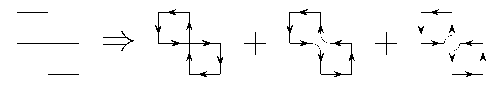
\includegraphics[width=80mm]{ising1}
  \caption{Переход от контуров к замкнутым путям}
  \label{fig:ising-1}
\end{figure}
Поэтому такие вклады надо брать с множителем $(-1)^{\nu(\Gamma)}$, где $\nu(\Gamma)$ - число самопересечений пути $\Gamma$.
Статсумма в высокотемпературном разложении \eqref{eq:108} дается выражением
\begin{equation}
  \label{eq:113}
  Z=(\ch K)^M 2^N\sum_c \kappa^{l[c]}.
\end{equation}
Обозначим сумму через $\Sigma=\sum_c \kappa^{l[c]}$. Перепишем её через сумму по путям
\begin{equation}
  \label{eq:114}
  \Sigma=\sum_{\Gamma}(-1)^{\nu(\Gamma)} \kappa^{l[\Gamma]}
\end{equation}
Воспользуемся следующим утверждением, доказательство которого оставляется в качестве упражнения. Для любой связной замкнутой петли на плоскости с $\nu$ самоперечечениями и полным углом поворота $2\pi(n+1)$ (при ее обходе) верно равенство
\begin{equation}
  \label{eq:115}
  (-1)^{\nu}=(-1)^n.
\end{equation}
Сопоставим каждому узлу в пути $\Gamma$ с углом поворота $\varphi$ в нем ($0,\pm \pi/2$) множитель $e^{\frac{i\varphi}{2}}$. Тогда после обхода петли полный множитель будет равен $(-1)^{\nu+1}$. Для несвязного пути, состоящего из $s$ компонент --- $(-1)^{m+s}$, где $m=\sum \nu$. То есть если ввести для пути $\Gamma$ общий множитель $s(\Gamma)$, то $\Sigma$ можно переписать в виде
\begin{equation}
  \label{eq:116}
  \Sigma=\sum_{\Gamma}(-1)^{s(\Gamma)}\prod_{j\in \Gamma} e^{\frac{i\varphi_j}{2}}\kappa^{l[\Gamma]}
\end{equation}
Обозначим через $F^{(1)}_l$ сумму по всем однокомпонентным петлям длины $l$, через $F^{(2)}_l$ --- двухкомпонентным и так далее.
\begin{equation}
  \label{eq:117}
  F^{(1)}_l=\sum_{\Gamma:l[\Gamma]=l} \prod_{j\in \Gamma} e^{\frac{i\varphi_j}{2}}.
\end{equation}
Тогда $F_l^{(2)}$ можно вычислить через $F^{(1)}$:
\begin{equation}
  \label{eq:118}
  F^{(2)}_l=\frac{1}{2!}\sum_{l_1,l_2:l_1+l_2=l} F^{(1)}_{l_1} F^{(1)}_{l_2}
\end{equation}
Аналогично
\begin{equation}
  \label{eq:119}
  F^{(s)}_l=\frac{1}{s!}\sum_{l_1,\dots l_s:l_1+\dots+l_s=l} F^{(1)}_{l_1}\dots F^{(1)}_{l_s}
\end{equation}
Теперь мы можем выразить $\Sigma$ через $F^{(1)}$:
\begin{equation}
  \label{eq:120}
  \Sigma=\sum_{s=0}^{\infty}\frac{1}{s!}\sum_{l_1\dots l_s=1}^{\infty} \kappa^{l_1+\dots+l_s}F^{(1)}_{l_1} \dots F^{(1)}_{l_s}=
  \sum_{s=0}^{\infty}\frac{1}{s!}\left(\sum_{l=1}^{\infty} \kappa^{l}F^{(1)}_{l} \right)^s =\exp\left(-\sum_{l=1}^{\infty} \kappa^l F_l\right)
\end{equation}
Петли с числом узлов больше $N$ не дают вклада, так как содержат повторяющиеся ребра и поэтому сократятся (Смотри рисунок \ref{fig:ising-2}).
\begin{figure}[h!tb]
  \centering
  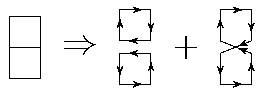
\includegraphics[width=40mm]{ising2}
  \caption{Сокращение путей с повторяющимися ребрами}
  \label{fig:ising-2}
\end{figure}
Наша задача свелась к вычислению $F_l$. Рассмотрим произвольную вершину с координатами $(n,m)$. Пронумеруем направления выхода из нее индексом $\nu=1,2,3,4$ против часовой стрелки. Обозначим через $W_l (n,m,\nu|n_0,m_0,\nu_0)$ сумму по всем путям длины $l$, соединяющим вершины $(n_0,m_0)$ и $(n,m)$. Первый шаг пути в направлении $\nu_0$. Учитываются множители $e^{\frac{i\varphi}{2}}$ начиная с узла, следующего за $(n_0,m_0)$ и заканчивая узлом $(n,m)$. Последний шаг пути не должен быть в направлении, противоположном $\nu$. Тогда $F_l$ можно записать как сумму $W_l(n,m,\nu|n,m,\nu)$ по всем вершинам решетки. Каждая петля при этом будет учтена $2l$ раз, так как у нее $l$ возможных вершин начала и два возможных направления.
\begin{equation}
  \label{eq:121}
  F_l=\frac{1}{2l}\sum_{(n,m)\in \mathcal{L}} \sum_{\nu=1,2,3,4} W_l(n,m,\nu|n,m,\nu)
\end{equation}
Если мы зафиксируем начальную вершину путей $(n_0,m_0,\nu_0)$, то сумму по путям длины $l+1$ можно выразить через сумму по путям длины $l$. В вершину $(n,m,1)$ пути могут входить с направлений $2,3,4$, то есть последний шаг может быть из вершины $(n-1,m)$ в направлении $1$, из вершины $(n,m-1)$ в направлении $2$ и из вершины $(n,m-1)$ в направлении $4$.
Аналогично для других направлений. Тогда
\begin{equation}
  \label{eq:122}
\begin{array}{l}
W_{l+1}(n,m,1)=W_l(n-1,m,1)+e^{-i\pi/4} W_l(n,m-1,2)+e^{i\pi/4}W_l(n,m-1,4)\\
W_{l+1}(n,m,2)=e^{i\pi/4}W_l(n-1,m,1)+W_l(n,m-1,2)+e^{i\pi/4}W_l(n+1,m,3)\\
W_{l+1}(n,m,3)=e^{i\pi/4}W_l(n,m-1,2)+W_l(n+1,m,3)+e^{-i\pi/4}W_l(n,m+1,4)\\
W_{l+1}(n,m,4)=e^{-i\pi/4}W_l(n-1,m,1)+e^{i\pi/4}W_l(n+1,m,3)+W_l(n,m+1,4)\\
\end{array}
\end{equation}
Эти рекуррентные соотношения можно переписать в матричном виде, если ввести матрицу коэффициентов $\Lambda$:
\begin{equation}
  \label{eq:124}
  W_{l+1}(n,m,\nu)=\sum_{p,q,\mu}\Lambda(n,m,\nu|t,u,\mu) W_l(t,u,\mu)
\end{equation}
Если вершины $(t,u)$ и $(n,m)$ не являются соседними, то $\Lambda(n,m,\nu|p,q,\mu)=0$. Матрица $\Lambda$ не зависит от начала пути. $W_{l+1}=\Lambda W_l$, поэтому мы $F_l$ дается следом $l$-той степени $\Lambda$:
\begin{equation}
  \label{eq:125}
  F_l=\frac{1}{2l}\mathrm{Tr} W_l=\frac{1}{2l}\mathrm{Tr} \Lambda^l W_0
\end{equation}
Но матрица $W_0=I$ (единичной матрице), поэтому
\begin{equation}
  \label{eq:126}
  F_l=\frac{1}{2l}\mathrm{Tr} \Lambda^l =\frac{1}{2l} \sum_k (\lambda_k)^l,
\end{equation}
где $\lambda_k$ - собственные значения матрицы $\Lambda$. Подставим выражение \eqref{eq:126} в формулу \eqref{eq:120}:
\begin{multline}
  \label{eq:127}
  \Sigma=\exp\left(-\sum_{l=0}^{\infty} \frac{\kappa^l}{2l}\mathrm{Tr}\Lambda^l\right)=\exp\left(-\frac{1}{2}\sum_k \sum_{l=0}^{\infty} \frac{(\kappa\lambda_k)^l}{l}\right)=\\
  \exp\left(\frac{1}{2}\sum_k \ln(1-\kappa\lambda_k)\right)=\prod_k(1-\kappa\lambda_k)^{1/2}=(\det(I-\kappa\Lambda))^{1/2}
\end{multline}
Чтобы вычислить детерминант сделаем дискретное преобразование Фурье:
\begin{equation}
  \label{eq:128}
  W_{l}(n,m,\nu)=\sum_{p_1,p_2} \tilde{W}_l(p_1,p_2,\nu) e^{\frac{2\pi i (p_1n+p_2m)}{\sqrt N}}
\end{equation}
В импульсном представлении матрица $\Lambda$ будет иметь блочно-диагональный вид
\begin{equation}
  \label{eq:129}
  \Lambda(p_1,p_2,\mu|q_1,q_2,\nu)=\delta_{p,q}\Lambda_p (\mu,\nu),
\end{equation}
где
\begin{equation}
  \label{eq:130}
  \Lambda_p(\mu,\nu)=
  \begin{pmatrix}
    e^{\frac{2\pi i p_1}{\sqrt N}} & e^{\frac{2\pi i p_2}{\sqrt N}} e^{-\frac{i\pi}{4}} & 0 & e^{\frac{2\pi i p_2}{\sqrt N}} e^{\frac{i\pi}{4}} \\
    e^{\frac{2\pi i p_1}{\sqrt N}} e^{\frac{i\pi}{4}} & e^{\frac{2\pi i p_2}{\sqrt N}} & e^{-\frac{2\pi i p_1}{\sqrt N}} e^{-\frac{i\pi}{4}} & 0 \\
    0 & e^{\frac{2\pi i p_2}{\sqrt N}} e^{\frac{i\pi}{4}} & e^{-\frac{2\pi i p_1}{\sqrt N}} & e^{-\frac{2\pi i p_2}{\sqrt N}} e^{-\frac{i\pi}{4}} \\
    e^{\frac{2\pi i p_1}{\sqrt N}} e^{-\frac{i\pi}{4}} & 0 & e^{\frac{2\pi i p_1}{\sqrt N}} e^{\frac{i\pi}{4}} & e^{-\frac{2\pi i p_2}{\sqrt N}}
  \end{pmatrix}
\end{equation}
Матрица $I-\kappa\Lambda$ тоже имеет блочный вид с блоками
\begin{equation}
  \label{eq:131}
  \begin{pmatrix}
    1-\kappa e^{\frac{2\pi i p_1}{\sqrt N}} & e^{\frac{2\pi i p_2}{\sqrt N}} e^{-\frac{i\pi}{4}} & 0 & e^{\frac{2\pi i p_2}{\sqrt N}} e^{\frac{i\pi}{4}} \\
    e^{\frac{2\pi i p_1}{\sqrt N}} e^{\frac{i\pi}{4}} & 1-\kappa e^{\frac{2\pi i p_2}{\sqrt N}} & e^{-\frac{2\pi i p_1}{\sqrt N}} e^{-\frac{i\pi}{4}} & 0 \\
    0 & e^{\frac{2\pi i p_2}{\sqrt N}} e^{\frac{i\pi}{4}} & 1-\kappa e^{-\frac{2\pi i p_1}{\sqrt N}} & e^{-\frac{2\pi i p_2}{\sqrt N}} e^{-\frac{i\pi}{4}} \\
    e^{\frac{2\pi i p_1}{\sqrt N}} e^{-\frac{i\pi}{4}} & 0 & e^{\frac{2\pi i p_1}{\sqrt N}} e^{\frac{i\pi}{4}} & 1- \kappa e^{-\frac{2\pi i p_2}{\sqrt N}}
  \end{pmatrix}.
\end{equation}
В результате вычисления детерминанта получаем
\begin{eqnarray}
  \label{eq:132}
  \Sigma=\prod_{p_1,p_2} D^{1/2}_{p}\\
  D_p=(1+\kappa^2)^2 -2\kappa (1-\kappa^2)\left( \cos \frac{2\pi p_1}{\sqrt N} +\cos \frac{2\pi p_2}{\sqrt N}\right)
\end{eqnarray}
В результате выражение для статсуммы имеет вид
\begin{equation}
  \label{eq:133}
  Z_N=(2\ch^2 K)^N \prod_{p_1,p_2}D_p^{1/2}.
\end{equation}
Исследуем критическое поведение. Вычислим для этого удельную свободную энергию:
\begin{equation}
  \label{eq:134}
  f=-T \lim_{N\to \infty}\frac{Z_N}{N}=-T \lim_{N\to \infty} \left(\ln (2\ch^2 K)+\frac{1}{2N}\sum_p \ln D_p\right)
\end{equation}
В термодинамическом пределе $N\to \infty$ значения импульса покрывают всю ось, поэтому сумма переходит в интеграл. Мы сделаем замену переменных
\begin{eqnarray}
  \label{eq:135}
  w_1=\frac{2\pi p_1}{\sqrt N}\quad  w_2=\frac{2\pi p_2}{\sqrt N},\quad w_{1,2}\in [0;2\pi]\\
  dp_1 dp_2=\frac{N}{(2\pi)^2} dw_1 dw_2
\end{eqnarray}
Вспомним, что $\kappa=\th K$, поэтому
\begin{equation}
  \label{eq:136}
  -\ln(2\ch^2 K)=\ln\left(\frac{1-\kappa^2}{2}\right)
\end{equation}
Нам будет удобно переписать $D_p$  в виде
\begin{equation}
  \label{eq:137}
  D_p=(\kappa^2+2\kappa -1)^2 +4\kappa (1-\kappa^2) \left(\sin^2 \frac{w_1}{2} +\sin^2 \frac{w_2}{2}\right)
\end{equation}
Тогда свободная энергия дается интегралом
\begin{multline}
  \label{eq:138}
  f=T\ln\left(\frac{1-\kappa^2}{2}\right)-\\
  -\frac{T}{8\pi^2}\int_0^{2\pi}\int_0^{2\pi}\ln\left((\kappa^2 +2\kappa-1)^2 +4\kappa (1-\kappa^2)\left(\sin^2 \frac{w_1}{2}+\sin^2\frac{w_2}{2}\right)\right) dw_1 \;dw_2
\end{multline}
В критической точке должна быть расходимость. Интеграл может иметь особую точку только при $(\kappa^2 +2\kappa-1)^2 +4\kappa (1-\kappa^2)\left(\sin^2 \frac{w_1}{2}+\sin^2\frac{w_2}{2}\right)=0$. Это выражение имеет минимум при $w_1=w_2=0$. Тогда при $\kappa^2+2\kappa-1=0$ интеграл расходится, что соответствует критической точке.
\begin{equation}
  \label{eq:139}
  \kappa_c=\sqrt 2 -1
\end{equation}
В критической точке основной вклад в интеграл дает окрестность $w_1=w_2=0$, введем
\begin{equation}
  \label{eq:140}
  \epsilon=\kappa-\kappa_c
\end{equation}
Тогда около критической точки свободная энергия ведет себя как
\begin{equation}
  \label{eq:141}
  f=g(\epsilon)-\frac{T}{8\pi^2}\int_{0}^{2\pi}\int_0^{2\pi}\ln \left( c\epsilon^2 +A(\epsilon)(w_1^2+w_2^2)\right)dw_1\;dw_2.
\end{equation}
Здесь $g(\epsilon), A(\epsilon)$ - регулярные функции. Если взять интеграл, то
\begin{equation}
  \label{eq:142}
  f\approx g_1 (\epsilon)+c\epsilon^2 \ln(e)
\end{equation}
Тогда для теплоемкости имеем
\begin{equation}
  \label{eq:143}
  c\propto \ln|T-T_c|
\end{equation}
То есть мы подтвердили, что критический индекс $\alpha=0$ (см. таблицу \ref{tab:diagrams}). Вычисление других критических индексов также возможно, но сопряжено с техническими трудностями. Мы не будем его проделывать, так как в следующих лекциях мы легко сможем вычислить корреляторы из конформной теории поля.
\section{Лекция 7. Конформная группа.}
\label{sec:lecture-7}

Построение Каданова-Вильсона (см. лекцию \ref{sec:kadanoff-procedure}) обосновало нам масштабную инвариантность модели Изинга. Сейчас мы обсудим, какие ограничения накладывает на теорию конформная инвариантность, а затем покажем, что в двух измерениях она следует из масштабной, трансляционной и вращательной инвариантностей.

Сперва рассмотрим конформную группу в произвольном числе измерений $d$. Метрический тензор обозначим через $g_{\mu\nu},\; \mu,\nu=1,\dots,d$. Конформными называются преобразования $x\to x'$, сохраняющие метрический тензор с точностью до масштаба:
\begin{equation}
  \label{eq:123}
  g'_{\mu\nu}(x')=\Lambda(x) g_{\mu\nu}(x).
\end{equation}
Заметим, что группа Пуанкаре является подгруппой конформной группы с $\Lambda(x)=1$, а также что конформные преобразования сохраняют углы. 

Рассмотрим инфинитезимальные преобразования
\begin{equation}
  \label{eq:144}
  x^{\mu}\to x'^{\mu}=x^{\mu}+\epsilon^{\mu}.
\end{equation}
Метрический тензор преобразуется следующим образом:
\begin{equation}
  \label{eq:145}
  g'_{\mu\nu}=\frac{\partial x^{\alpha}}{\partial x'^{\mu}}\frac{\partial x^{\beta}}{\partial x'^{\nu}} g_{\alpha\beta}=(\delta^{\alpha}_{\mu}-\partial_{\mu}\epsilon^{\alpha})(\delta^{\beta}_{\nu}-\partial_{\nu} \epsilon^{\beta})g_{\alpha\beta}=g_{\mu\nu}-(\partial_{\mu}\epsilon_{\nu}+\partial_{\nu}\epsilon_{\mu})
\end{equation}
Перепишем условие (\ref{eq:123})в таком виде:
\begin{equation}
  \label{eq:146}
  g'_{\mu\nu}(x')=g_{\mu\nu}(x)-f(x)g_{\mu\nu}(x)
\end{equation}
Отсюда вытекает условие на вид преобразований:
\begin{equation}
  \label{eq:147}
  \partial_{\mu}\epsilon_{\nu}+\partial_{\nu}\epsilon_{\mu}=f(x)g_{\mu\nu}(x).
\end{equation}
Для простоты рассмотрим преобразования, действующие на плоскую метрику $g_{\mu\nu}(x)=\eta_{\mu\nu}$, кроме того, с учетом приложений к статистической физике, будем работать в евклидовом пространстве, а не в пространстве Минковского. Так что $\eta=\mathrm{diag}(1,1,\dots,1),\quad \eta_{\mu\nu}=\delta_{\mu\nu}$. В этом случае условие \eqref{eq:147} перепишется в простом виде
\begin{equation}
  \label{eq:148}
  f(x)=\frac{2}{d}\partial_{\rho}\epsilon^{\rho}.
\end{equation}
Теперь подставим $g_{\mu\nu}=\eta_{\mu\nu}$ в уравнение \eqref{eq:147} и продиффернцируем:
\begin{equation}
  \label{eq:149}
  \partial_{\rho} \partial_{\mu}\epsilon_{\nu}+\partial_{\rho}\partial_{\nu}\epsilon_{\mu}=\eta_{\mu\nu}\partial_{\rho} f.
\end{equation}
Переставим два раза значки и скомбинируем три уравнения в одно:
\begin{equation}
  \label{eq:150}
  2\partial_{\mu}\partial_{\nu}\epsilon_{\rho}=\eta_{\mu\rho}\partial_{\nu} f+\eta_{\nu\rho}\partial_{\mu}f-\eta_{\mu\nu}\partial_{\rho}f
\end{equation}
Свернем это уравнение с $\eta^{\mu\nu}$ и получим
\begin{equation}
  \label{eq:151}
  2\partial^2 \epsilon_{\rho}=(2-d)\partial_{\rho}f
\end{equation}
Теперь продифференцируем его по $x^{\nu}$ и поменяем значок $\rho$ на $\mu$:
\begin{equation}
  \label{eq:152}
  2\partial^2 \partial_{\nu} \epsilon_{\mu}=(2-d)\partial_{\mu}\partial_{\nu} f
\end{equation}
Сравним полученное равенство с результатом применения оператора $\partial^2$ к уравнению \eqref{eq:149}:
\begin{equation}
  \label{eq:153}
  \partial^2 \partial_{\mu}\epsilon_{\nu}+\partial^2 \partial_{\nu}\epsilon_{\mu}=\eta_{\mu\nu}\partial^2 f
\end{equation}
Из равенств \eqref{eq:152}, \eqref{eq:153} следует, что
\begin{equation}
  \label{eq:154}
  (2-d)\partial_{\mu}\partial_{\nu}f=\eta_{\mu\nu}\partial^2 f.
\end{equation}
Свернув с $\eta^{\mu\nu}$ получим
\begin{equation}
  \label{eq:155}
  (d-1)\partial^2 f =0.
\end{equation}
Сразу можно отметить, что при $d=1$ любое гладкое преобразование будет конформным. Рассмотрим случай $d\geq 3$. Функция $f(x)$ должна иметь вид
\begin{equation}
  \label{eq:156}
  f(x)=A+B_{\mu}x^{\mu}.
\end{equation}
Тогда из \eqref{eq:148} получаем для $\epsilon$
\begin{equation}
  \label{eq:157}
  \epsilon_{\mu}=a_{\mu}+b_{\mu\nu}x^{\nu} +c_{\mu\nu\rho}x^{\nu}x^{\rho},\quad c_{\mu\nu\rho}=c_{\mu\rho\nu}
\end{equation}
Так как равенства \eqref{eq:147}, \eqref{eq:148}, \eqref{eq:150} должны выполняться для любых $x^{\mu}$, то мономы в $\epsilon$ можно рассматривать независимо. На $a_{\mu}$ не возникает никаких ограничений. Этот член соответствует трансляциям. Теперь подставляем линейный член в \eqref{eq:147}, \eqref{eq:148} и получаем условие
\begin{equation}
  \label{eq:158}
  b_{\mu\nu}+b_{\nu\mu}=\frac{2}{d}b^{\lambda}_{\lambda}\eta_{\mu\nu}
\end{equation}
То есть $b_{\mu\nu}$ можно записать в виде
\begin{equation}
  \label{eq:159}
  b_{\mu\nu}=\alpha \eta_{\mu\nu} +m_{\mu\nu},\quad m_{\mu\nu}=-m_{\nu\mu}
\end{equation}
Первый член соответствует масштабному преобразованию, а второй - повороту. 
В результате подстановки квадратичного члена $\epsilon$ в \eqref{eq:148}, \eqref{eq:150} получаем следующее условие на $c_{\mu\nu\rho}$:
\begin{equation}
  \label{eq:160}
  c_{\mu\nu\rho}=\eta_{\mu\rho} h_{\nu} +\eta_{\mu\nu}h_{\rho}-\eta_{\nu\rho}h_{\mu}, \quad h_{\mu}=\frac{1}{d} c^{\alpha}_{\alpha\mu}
\end{equation}
Ему соответствует преобразование
\begin{equation}
  \label{eq:161}
  x'^{\mu}=x^{\mu}+2 (x^{\nu}h_{\nu})x^{\mu} -h^{\mu} x^{\nu}x_{\nu}
\end{equation}
Такое преобразование называется специальным конформным преобразованием.
Это преобразование можно естественно интерпретировать, если переписать в виде
\begin{equation}
  \label{eq:162}
  \frac{x'^{\mu}}{x'^2}=\frac{x^{\mu}}{x^2}-h^{\mu}.
\end{equation}
Видно, что специальное конформное преобразование --- это инверсия, трансляция и обратная инверсия. 

Соответствующие конченые конформные преобразования имеют вид
\begin{eqnarray}
  \label{eq:163}
  x'^{\mu}=x^{\mu}+a^{\mu}&\quad \mbox{--- трансляция}\\
  x'{\mu}=\alpha x^{\mu} &\quad \mbox{--- растяжение}\\
  x'^{\mu}=m^{\mu}_{\nu} x^{\nu} &\quad \mbox{--- поворот}\\
  x'^{\mu}=\frac{x^{\mu}-h^{\mu}x^2}{1-2h_{\mu}x^{\mu}+h^2 x^2}  & \quad \begin{array}{c}\mbox{--- специальное конформное}\\ \mbox{ преобразование}\end{array}
\end{eqnarray}

Теперь выпишем вид генераторов конформных преобразований для скалярного поля. 
Напомним, что при произвольном конечном преобразовании скалярное поле преобразуется как
\begin{equation}
  \label{eq:164}
  \Phi'(x')=F(\Phi(x)).
\end{equation}
При соответствующем инфинитезимальном преобразовании
\begin{equation}
  \label{eq:165}
  x'^{\mu}=x^{\mu}+\omega_a \frac{\delta x^{\mu}}{\delta \omega_a}
\end{equation}
скалярное поле преобразуется так:
\begin{equation}
  \label{eq:166}
  \Phi'(x')=\Phi(x)+\omega_a \frac{\delta F}{\delta \omega_a} (x).
\end{equation}
Генератор преобразования определяется следующим равенством:
\begin{equation}
  \label{eq:167}
  \delta_{\omega} \Phi(x)=\Phi'(x)-\Phi(x)\equiv -i\omega_a G_a \Phi(x)
\end{equation}
(здесь нет суммирования по $a$). Из \eqref{eq:166} получаем действие генератора на скалярное поле:
\begin{equation}
  \label{eq:168}
  iG_a \Phi=\frac{\delta x^{\mu}}{\delta\omega_a} \partial_{\mu}\Phi-\frac{\delta F}{\delta \omega_a}
\end{equation}

Если мы предположим, что поле $\Phi$ такое поле, которое не меняется при конформных преобразованиях, то есть $F(\Phi)=\Phi$, то мы получим следующий вид для генераторов:
\begin{eqnarray}
  \label{eq:169}
  \mbox{трансляция} & \quad P_{\mu}=-i\partial_{\mu}\\
  \mbox{поворот} & \quad L_{\mu\nu}=i(x_{\mu}\partial_{\nu}-x_{\nu}\partial{\mu})\\
  \mbox{растяжение}& \quad D=-ix^{\mu}\partial_{\mu}\\
  \begin{array}{r}
  \mbox{специальное конформное}    \\
  \mbox{преобразование}
  \end{array}
  & \quad K_{\mu}=-i(2x_{\mu}x^{\nu}\partial_{\nu}-x^2\partial_{\mu})
\end{eqnarray}
Отсюда легко найти коммутационные соотношения алгебры конформных преобразований в случае $d\geq 3$:
\begin{eqnarray}
  \label{eq:170}
  \left[D,P_{\mu}\right]=i P_{\mu}\\
  \left[D,K_{\mu}\right]=-i K_{\mu}\\
  \left[K_{\mu},P_{\nu}\right]=2i (\eta_{\mu\nu}D - L_{\mu\nu})\\
  \left[K_{\rho},L_{\mu\nu}\right]=i(\eta_{\rho\mu}P_{\nu}-\eta_{\rho\nu}P_{\mu})\\
 \left[L_{\mu\nu},L_{\rho\sigma}\right]=i(\eta_{\nu\rho}L_{\mu\sigma}+\eta_{\mu\sigma}L_{\nu\rho}-\eta_{\mu\rho}L_{\nu\sigma}-\eta_{\nu\sigma}L_{\mu\rho})
\end{eqnarray}
Остальные коммутаторы равны нулю.
Чтобы понять, о какой алгебре идет речь, переопределим генераторы следующим образом. Введем генераторы $J_{ab}, \; a,b=-1,0,\dots,d, J_{ab}=-J_{ba}$:
\begin{eqnarray}
  \label{eq:171}
  J_{\mu\nu}=L_{\mu\nu}\\
  J_{-1,0}=D\\
  J_{-1,\mu}=\frac{1}{2}(P_{\mu}-K_{\mu})\\
  J_{0,\mu}=\frac{1}{2}(P_{\mu}+K_{\mu})
\end{eqnarray}
Коммутационные соотношения для таких генераторов запишутся в виде
\begin{equation}
  \label{eq:172}
  \left[J_{ab},J_{cd}\right]=i(\eta_{ad}J_{bc}+\eta_{bc}J_{ad}-\eta_{ac}J_{bd}-\eta_{bd}J_{ac}),
\end{equation}
где $\eta_{ab}=\mathrm{diag}(-1,1,\dots,1)$. Видно, что мы получили алгебру $so(d+1,1)$. В случае пространства Минковского была бы $so(d,2)$.
\section{Лекция 8}
\label{sec:lecture-8}

\subsection{Инварианты}
\label{sec:invariants}

Обсудим, какой вид могут иметь простейшие инварианты --- $N$-точечные функции $\Gamma(x_1,\dots,x_N)$. В силу трансляционной инвариантности они могут зависеть только от модуля разности $|\vec x_i-\vec x_j|$.  Масштабная инвариантность может сохраняться только отношениями
\begin{equation}
  \label{eq:173}
  \frac{|\vec x_i-\vec x_j|}{|\vec x_k -\vec x_l|}
\end{equation}
Но при специальных конформных преобразованиях
\begin{equation}
  \label{eq:174}
  |\vec x'_i-\vec x'_j|=\frac{|\vec x_i-\vec x_j|}{(1-2(\vec h,\vec x_i)+h^2x_i^2)^{1/2} (1-2(\vec h,\vec x_j)+h^2 x_j^2)^{1/2}}
\end{equation}
Поэтому не обойтись двумя или тремя точками и простейшие инварианты имеют вид
\begin{eqnarray}
  \label{eq:175}
  \frac{|\vec x_1-\vec x_2||\vec x_3-\vec x_4|}{|\vec x_1-\vec x_3||\vec x_{2}-\vec x_{4}|}\\
  \frac{|\vec x_1-\vec x_2||\vec x_3-\vec x_4|}{|\vec x_2-\vec x_3||\vec x_{1}-\vec x_{4}|}
\end{eqnarray}
Всего $N(N-3)/2$ вариантов для $N$ точек.

\subsection{Явный вид конформных преобразований полей в $d\geq 3$.}
\label{sec:conformal-transforms-explicit}

Покажем теперь, как преобразуются поля при конформных преобразованиях. Для этого используем метод индуцированных представлений, который можно легко объяснить на примере алгебры Пуанкаре. Сначала рассматриваем подалгебру, которая оставляет точку $x=0$ неподвижной. Это алгебра группы Лоренца или группы вращений в случае евклидова пространства. На поля в точке $x=0$ она действует своими матричными представлениями:
\begin{equation}
  \label{eq:176}
  L_{\mu\nu}\Phi(0)=S_{\mu\nu}\Phi(0)
\end{equation}
Затем мы пользуемся коммутационными соотношениями алгебры Пуанкаре и формулой Хаусдорфа
\begin{equation}
  \label{eq:177}
  e^{-A}B e^{A}=B+[B,A]+\frac{1}{2!}[[B,A],A]+\frac{1}{3!}[[[B,A],A],A]+\dots
\end{equation}
чтобы вычислить результат переноса в точку $x$:
\begin{multline}
  \label{eq:178}
  L_{\mu\nu}\Phi(x)=e^{ix^{\rho}P_{\rho}}L_{\mu\nu}e^{-i x^{\rho}P_{\rho}}\Phi(x)=\\
  (S_{\mu\nu}-x_{\mu}P_{\nu}+x_{\nu}P_{\mu})\Phi(x)=\\
  i(x_{\mu}\partial_{\nu}-x_{\nu}\partial_{\mu})\Phi(x)+S_{\mu\nu}\Phi(x)
\end{multline}
Для полной конформной группы подгруппа стабильности точки $x=0$ порождается поворотами, растяжениями и специальными конформными преобразованиями. Обозначим представление генераторов через $S_{\mu\nu}, \tilde \Delta, k_{\mu}$ соответственно. Они порождают матричное представление усеченной алгебры с коммутационными соотношениями
\begin{eqnarray}
  \label{eq:179}
  \left[\tilde\Delta,S_{\mu\nu}\right]=0\\
  \left[\tilde \Delta,k_{\mu}\right]=-i k_{\mu}\\
  \left[k_{\mu},k_{\nu}\right]=0\\
  \left[k_{\rho},S_{\mu\nu}\right]=i(\eta_{\rho\mu}k_{\nu}-\eta_{\rho\nu}k_{\mu})\\
  \left[S_{\mu\nu},S_{\rho\sigma}\right]=i(\eta_{\nu\rho}S_{\mu\sigma}+\eta_{\mu\sigma}S_{\nu\rho}-\eta_{\mu\rho}S_{\nu\sigma}-\eta_{\nu\sigma}S_{\mu\rho})
\end{eqnarray}
Трансляция генераторов дилатации и специальных конформных преобразований дается равенствами
\begin{eqnarray}
  \label{eq:180}
  e^{i x^{\rho}P_{\rho}}D e^{-i x^{\rho}P_{\rho}}=D+x^{\nu}P_{\nu}\\
  e^{i x^{\rho}P_{\rho}}K_{\mu} e^{-i x^{\rho}P_{\rho}}=K_{\mu}+2x_{\mu}D -2 x^{\nu}L_{\mu\nu}+2x_{\mu}(x^{\nu}P_{\nu})-x^{2 P_{\mu}}
\end{eqnarray}
В результате действие этих генераторов на поле имеет вид
\begin{eqnarray}
  \label{eq:181}
  D\Phi(x)=(-ix^{\nu}\partial_{\nu}+\tilde \Delta)\Phi(x)\\
  K_{\mu}\Phi(x)=(k_{\mu}+2x_{\mu}\tilde\Delta -x^{\nu}S_{\mu\nu}-2ix_{\mu}x^{\nu}\partial_{\nu}+ix^{2} \partial_{\mu})\Phi(x)
\end{eqnarray}
Если требовать, чтобы поле $\Phi(x)$ преобразовывалось по неприводимому представлению группы Лоренца, то по лемме Шура любая матрица, коммутирующая со всеми генераторами $S_{\mu\nu}$ пропорциональна единичной.  
\begin{mynote}
  
  {\it Лемма Шура}. Оператор, сплетающий неприводимые конечномерные представления группы Ли либо нулевой, либо обратим. Эта лемма доказывается в любом учебнике по теории групп Ли, например \cite{golod2001}. 

  {\it Следствие}. Оператор $B$, коммутирующий со всеми операторами конечномерного неприводимого представления, кратен единичному.

  {\it Доказательство}: рассмотрим оператор $B-\lambda I$, он тоже коммутирует со всеми операторами представления. Возьмем $\lambda=\lambda_1$, являющееся решением уравнения $\det (B-\lambda I)=0$. Тогда оператор $B-\lambda I$ вырожден, и по лемме Шура равен нулю. Следовательно $B\propto I$.
\end{mynote}

То есть $\tilde \Delta\propto I$ и $k_{\mu}=0$. Тогда $\tilde \Delta =-i \Delta I$, где $\Delta$ -- скейлинговая размерность поля $\Phi$, $\Phi'(\lambda x)=\lambda^{-\Delta}\Phi(x)$. Закон преобразования бесспинового поля $\varphi$ при конечных конформных преобразованиях
\begin{eqnarray}
  \label{eq:182}
  x\to x'\\
  \varphi(x)\to \varphi'(x')=\left|\frac{\partial x'}{\partial x}\right|^{-\Delta/d}\varphi(x)\\
  \left|\frac{\partial x'}{\partial x}\right|=\Lambda(x)^{-d/2}    \quad\mbox{--- якобиан преобразования}
\end{eqnarray}
Поля, которые так преобразуются, называются {\it квазипримарными}.

Заметим, что  вариация действия при конформных преобразованиях определяется тензором энергии импульса:
\begin{equation}
  \label{eq:183}
  \delta S=\int d^{d}x T^{\mu\nu}\partial_{\mu}\epsilon_{\nu}=\frac{1}{2} \int d^{d}x T^{\mu\nu}(\partial_{\mu}\epsilon_{\nu}-\partial_{\nu}\epsilon_{\mu})=\frac{1}{d}\int d^{d}x T^{\mu}_{\mu}\partial_{\rho}\epsilon^{\rho},
\end{equation}
где мы использовали равенства \eqref{eq:147}, \eqref{eq:148}. То есть бесследовость тензора энергии-импульса ведет к конформной инвариантности классической теории поля. В классической теории поля при наличии трансляционной, вращательной и масштабной инвариантности  тензор энергии-импульса часто можно переопределить так, чтобы он был бесследовым. То есть конформная инвариантность следует из трансляционной, вращательной и масштабной. В случае двумерной квантовой теории поля общего доказательства нет, но конформная инвариантность наблюдается во множестве моделей. 

\section{Лекция 9}
\label{sec:lecture-9}

\subsection{Корреляторы квазипримарных полей}
\label{sec:quasiprimary-correlators}

Теперь перейдем к квантовой теории поля. Рассмотрим коррелятор квазипримарных полей.
\begin{equation}
  \label{eq:184}
  \langle \varphi_{1}(x_{1}) \varphi_{2}(x_{2})\rangle = \frac{1}{Z} \int \mathcal{D} \Phi \varphi_{1}(x_{1})\varphi_{2}(x_{2}) e^{-S[\Phi]}
\end{equation}
Мы знаем, как преобразуется поле при конформных преобразованиях \eqref{eq:182}, поэтому коррелятор должен вести себя так:
\begin{equation}
  \label{eq:185}
  \langle \varphi_{1}(x_{1})\varphi_{2}(x_{2})\rangle = \left|\frac{\partial x'_{1}}{\partial x_{1}}\right|^{\frac{\Delta_{1}}{d}}\left| \frac{\partial x'_{2}}{\partial x_{2}}\right|^{\frac{\Delta_{1}}{d}} \langle \varphi_{1}(x'_{1})\varphi_{2}(x'_{2})\rangle .
\end{equation}
Из требования инвариантности коррелятора при поворотах и трансляциях получаем, что коррелятор может зависеть только от модуля разности $\left|x_{1}-x_{2}\right|$:
\begin{equation}
  \label{eq:186}
  \langle \varphi_{1}(x_{1}) \varphi_{2}(x_{2})\rangle = f(\left|x_{1}-x_{2}\right|)
\end{equation}
При масштабных преобразованиях $x\to \lambda x$ из \eqref{eq:185} получаем
\begin{equation}
  \label{eq:187}
   \langle \varphi_{1}(x_{1}) \varphi_{2}(x_{2})\rangle=\lambda^{\Delta_{1}+\Delta_{2}}  \langle \varphi_{1}(\lambda x_{1}) \varphi_{2}(\lambda x_{2})\rangle .
\end{equation}
То есть мы видим, что $ \langle \varphi_{1}(x_{1}) \varphi_{2}(x_{2})\rangle$ - однородная функция, $f(x)=\lambda^{\Delta_{1}+\Delta_{2}} f(\lambda x)$. Отсюда
\begin{equation}
  \label{eq:188}
   \langle \varphi_{1}(x_{1}) \varphi_{2}(x_{2})\rangle = \frac{C_{12}}{\left|x_{1}-x_{2}\right|^{\Delta_{1}+\Delta_{2}}}.
\end{equation}
Однако мы ещё не воспользовались инвариантностью коррелятора относительно специальных конформных преобразований. Подставим явный вид преобразований $\left|x_{1}-x_{2}\right|$ из \eqref{eq:174} и введем обозначение $\gamma_{i}=\left(1-2(h,x_{i})+h^{2}x_{i}^{2}\right)$, тогда
\begin{equation}
  \label{eq:189}
  \frac{C_{12}}{\left|x_{1}-x_{2}\right|^{\Delta_{1}+\Delta_{2}}}=\frac{C_{12}(\gamma_{1}\gamma_{2})^{(\Delta_{1}+\Delta_{2})/2}}{\gamma_{1}^{\Delta_{1}}\gamma_{2}^{\Delta_{2}} \left|x_{1}-x_{2}\right|}.
\end{equation}
Это равенство может выполняться только при $\Delta_{1}=\Delta_{2}$. В итоге для коррелятора
\begin{equation}
  \label{eq:190}
   \langle \varphi_{1}(x_{1}) \varphi_{2}(x_{2})\rangle =
   \begin{cases}
     \frac{C_{12}}{\left|x_{1}-x_{2}\right|^{2\Delta_{1}}} & \Delta_{1}=\Delta_{2}\\
     0 & \Delta_{1}\neq \Delta_{2}
   \end{cases}
\end{equation}
Вспомним, что для парной корреляционной функции мы вводили критический индекс $\eta$: $\Gamma(\vec n)\sim |\vec n|^{2-d-\eta}$. То есть для коррелятора квазипримарых полей
\begin{equation}
  \label{eq:191}
  \eta=2\Delta +2 -d.
\end{equation}

Аналогичный анализ можно провести для трехточечных функций. Из требований трансляционной и вращательной инвариантности имеем
\begin{equation}
  \label{eq:192}
  \langle \varphi_{1}(x_{1})\varphi_{2}(x_{2})\varphi_{3}(x_{3})\rangle=\frac{C^{abc}_{123}}{x_{12}^{a} x_{23}^{b}x_{13}^{c}},\quad a+b+c=\Delta_{1}+\Delta_{2}+\Delta_{3}.
\end{equation}
Здесь введено обозначение $x_{ij}=|x_{i}-x_{j}|$.
Из требования инвариантности при специальных конформных преобразованиях получаем
\begin{equation}
  \label{eq:193}
  \frac{C^{abc}_{123}}{x_{12}^{a} x_{23}^{b}x_{13}^{c}}=\frac{C^{abc}_{123}}{\gamma_{1}^{\Delta_{1}}\gamma_{2}^{\Delta_{2}}\gamma_{3}^{\Delta_{3}}}\frac{(\gamma_{1}\gamma_{2})^{a/2}(\gamma_{2}\gamma_{3})^{b/2}(\gamma_{1}\gamma_{3})^{c/2}}{x_{12}^{a} x_{23}^{b}x_{13}^{c}}
\end{equation}
Это равенство может выполняться только при
\begin{equation}
  \label{eq:194}
  \begin{array}{l}
    a+c=2\Delta_{1}\\
    a+b=2\Delta_{2}\\
    b+c=2\Delta_{3}
  \end{array}
\end{equation}
Отсюда сразу получаем, сто
\begin{equation}
  \label{eq:195}
  \begin{array}{l}
    a=\Delta_{1}+\Delta_{2}-\Delta_{3}\\
    b=\Delta_{2}+\Delta_{3}-\Delta_{1}\\
    c=\Delta_{3}+\Delta_{1}-\Delta_{2}.
  \end{array}
\end{equation}
В итоге для трехточечных функций имеем:
\begin{equation}
  \label{eq:196}
   \langle \varphi_{1}(x_{1})\varphi_{2}(x_{2})\varphi_{3}(x_{3})\rangle=\frac{C^{abc}_{123}}{x_{12}^{\Delta_{1}+\Delta_{2}-\Delta_{3}} x_{23}^{\Delta_{2}+\Delta_{3}-\Delta_{1}}x_{13}^{\Delta_{3}+\Delta_{1}-\Delta_{2}}}.
\end{equation}
Из четырех точек уже можно собрать инварианты \eqref{eq:175}, поэтому из требований конформной инвариантности для четырехточечной функции можно написать только
\begin{equation}
  \label{eq:197}
  \langle \varphi_{1}(x_{1})\varphi_{2}(x_{2})\varphi_{3}(x_{3})\varphi_{4}(x_{4})\rangle=f\left(\frac{x_{12}x_{34}}{x_{13}x_{24}}; \frac{x_{12}x_{34}}{x_{23}x_{14}}\right) \prod_{i<j}^{4}x_{ij}^{\Delta/3-\Delta_{i}-\Delta_{j}},\quad \Delta=\sum_{i=1}^{4}\Delta_{i}.
\end{equation}

\subsection{Тождества Уорда}
\label{sec:ward-identities}

Напомним, о чем идет речь. В произвольной теории поля с полями $\Phi(x)$ инфинитезимальное преобразование может быть записано при помощи генераторов
\begin{equation}
  \label{eq:198}
  \Phi'(x)=\Phi(x)-i\omega_{a} G_{a} \Phi(x)
\end{equation}
Вариация действия вычисляется через ток, соответствующий данному преобразовании:
\begin{equation}
  \label{eq:199}
  j^{\mu}_{a}=\left(\frac{\partial \mathcal{L} }{\partial (\partial_{\mu}\Phi)} \partial_{\nu}\Phi -\delta^{\mu}_{\nu}\mathcal{L}\right) \frac{\delta x^{\nu}}{\delta \omega_{a}} - \frac{\partial \mathcal{L} }{\partial (\partial_{\mu} \Phi)}\frac{\delta F}{\delta \omega_{a}}
\end{equation}
\begin{equation}
  \label{eq:200}
  \delta S =\int d^{d}x \partial_{\mu}j^{\mu}_{a} \omega_{a}
\end{equation}
Обозначим через $X$ произведение локальных полей, входящих в коррелятор
\begin{equation}
  \label{eq:201}
  X=\Phi(x_{1})\dots \Phi(x_{n}).
\end{equation}
Коррелятор дается функциональным интегралом
\begin{equation}
  \label{eq:202}
  \langle X\rangle = \frac{1}{Z}\int \mathcal{D} \Phi X e^{-S[\Phi]}
\end{equation}
Сделаем замену переменных $\Phi\to \Phi'$ в функциональном интеграле. При этом можно предполагать, что ``мера интегрирования'' не меняется $\mathcal{D}\Phi'=\mathcal{D}\Phi$ \cite{difrancesco1997cft}:
\begin{equation}
  \label{eq:203}
  \langle X\rangle = \frac{1}{Z} \int \mathcal{D} \Phi' (X+\delta X)e^{-S[\Phi]-\int d^{d}x \partial_{\mu}j^{\mu}_{a}\omega_{a}(x)}
\end{equation}
Раскладываем выражение в ряд до первого порядка по $\omega_{a}(x)$:
\begin{equation}
  \label{eq:204}
  \langle X\rangle=\frac{1}{Z} \left( \int \mathcal{D} \Phi X e^{-S[\Phi]}+\int \mathcal{D} \Phi \delta X e^{-S[\Phi]} -\int \mathcal{D}\Phi \int d^{d}x \partial_{\mu}j^{\mu}_{a}\omega_{a}(x) X e^{-S[\Phi]}\right)
\end{equation}
В результате имеем
\begin{equation}
  \label{eq:205}
  \langle \delta X\rangle=\int d^{d}x \partial_{\mu}\langle j^{\mu}_{a}(x) X\rangle \omega_{a}(x)
\end{equation}
С другой стороны, мы можем вычислить $\langle\delta X\rangle$ используя \eqref{eq:198}:
\begin{multline}
  \label{eq:206}
  \langle\delta X\rangle=-i\sum_{i=1}^{n}\langle \Phi(x_{1})\dots G_{a} \Phi(x_{i}) \dots \Phi(x_{n})\rangle \omega_{a}(x_{i})=\\
  -i \int d^{d}x \omega_{a}(x) \sum_{i=1}^{n} \langle \Phi(x_{1}) \dots G_{a} \Phi(x_{i}) \dots \Phi(x_{n})\rangle \delta (x-x_{i})
\end{multline}
Окончательно общий вид тождеств Уорда выглядит следующим образом:
\begin{equation}
  \label{eq:207}
  \partial_{\mu}\langle j^{\mu}_{a}\Phi(x_{1}) \dots \Phi(x_{n})\rangle=-i\sum_{i=1}^{n}\delta (x-x_{i}) \langle\Phi(x_{1})\dots G_{a} \Phi(x_{i})\dots \Phi(x_{n})\rangle
\end{equation}
Рассмотрим некоторые примеры, которые понадобятся нам для конформной теории. Мы используем полученный нами явный вид генераторов \eqref{eq:169}.

Тождество Уорда для трансляций:
\begin{equation}
  \label{eq:208}
  \partial_{\mu}\langle T^{\mu}_{\nu} X\rangle =-i \sum_{i} \delta(x-x_{i}) \frac{\partial}{\partial x_{i}^{\nu}} \langle X \rangle
\end{equation}
Теперь рассмотрим вращения. Если тензор энергии-импульса симметризован (это можно сделать в большинстве случаев), то отвечающий вращениям ток дается выражением
\begin{equation}
  \label{eq:209}
  j^{\mu\nu\rho}=T^{\mu\nu}x^{\rho}-T^{\mu\rho}x^{\nu}.
\end{equation}
Тогда тождество Уорда может быть записано в виде
\begin{equation}
  \label{eq:210}
  \partial_{\mu}\langle (T^{\mu\nu}x^{\rho}-T^{\mu\rho}x^{\nu}) X\rangle=\sum_{i }\delta(x-x_{i}) \left( (x^{\nu}_{i}\partial^{\rho}_{i}-x^{\rho}_{i}\partial^{\nu}_{i})\langle X\rangle-i S^{\nu\rho}_{i}\langle X\rangle\right).
\end{equation}
Его можно упростить с использованием тождества для трансляций \eqref{eq:208}:
\begin{equation}
  \label{eq:211}
  \langle (T^{\rho\nu}-T^{\nu\rho}) X\rangle=-i \sum_{i} \delta(x-x_{i}) S^{\nu\rho}_{i}\langle X\rangle.
\end{equation}
Тензор энергии-импульса в квантовой теории симметричен в корреляционных функциях, если его положение не совпадает с положениями других полей в корреляторе. 

Наконец, для масштабных преобразований ток имеет вид $T^{\mu}_{\nu}x^{\nu}$, действие генератора дается выражением \eqref{eq:181} и тождества Уорда выглядят так:
\begin{equation}
  \label{eq:212}
  \partial_{\mu}\langle T^{\mu}_{\nu} x^{\nu} X\rangle=-\sum_{i} \delta(x-x_{i}) \left( x^{\nu}_{i}\frac{\partial}{\partial x^{\nu}_{i}} \langle X\rangle+\Delta_{i} \langle X\rangle\right) 
\end{equation}
Его тоже можно упростить:
\begin{equation}
  \label{eq:213}
  \langle T^{\mu}_{\mu} X \rangle = -i \sum_{i} \delta(x-x_{i}) \Delta_{i}\langle X\rangle
\end{equation}

\subsection{О бесследовости тензора энергии-импульса.}
\label{sec:tracelessness}

В некоторых теориях из масштабной, вращательной и трансляционной инвариантности автоматически следует конформная инвариантность. Как мы знаем, конформная инвариантность соответствует бесследовости тензора энергии-импульса. Общего доказательства конформной инвариантности для масштабно-, трансляционно- и вращательно-инвариантных теорий не существует даже для двумерного случая, однако мы можем показать, что вакуумное среднее квадрата следа тензора энергии-импульса в этом случае равно нулю.

Для этого рассмотрим функцию Швингера
\begin{equation}
  \label{eq:214}
  S_{\mu\nu\rho\sigma}=\langle T_{\mu\nu}(x) T_{\rho\sigma}(0)\rangle.
\end{equation}
Из симметричности тензора энергии-импульса
\begin{equation}
  \label{eq:215}
  S_{\mu\nu\rho\sigma}=S_{\nu\mu\rho\sigma}=S_{\mu\nu\sigma\rho}=S_{\nu\mu\sigma\rho}
\end{equation}
Теперь воспользуемся трансляционной инвариантностью:
\begin{equation}
  \label{eq:216}
  S_{\mu\nu\rho\sigma}=\langle T_{\mu\nu}(0)T_{\rho\sigma}(-x)\rangle =\langle T_{\rho\sigma}(-x) T_{\mu\nu}(0)\rangle = S_{\rho\sigma\mu\nu}(-x).
\end{equation}
Если в теории сохраняется четность, то $S_{\mu\nu\rho\sigma}(x)=S_{\rho\sigma\mu\nu}(x)$. В силу масштабной инвариантности $T_{\mu\nu}$ имеет скейлинговую размерность 2, так как является плотностью. Следовательно функция Швингера при масштабных преобразованиях ведет себя так:
\begin{equation}
  \label{eq:217}
  S_{\mu\nu\rho\sigma}(\lambda x)=\lambda^{-4} S_{\mu\nu\rho\sigma}(x)
\end{equation}
Теперь можно записать общий вид функции Швингера:
\begin{multline}
  \label{eq:218}
  S_{\mu\nu\rho\sigma}(x)=(x^{2})^{-4} \left( A_{1}g_{\mu\nu} g_{\rho\sigma} (x^{2})^{2} + A_{2} (g_{\mu\rho}g_{\nu\sigma}\right. +\\
  \left. g_{\mu\sigma}g_{\nu\rho}) (x^{2})^{2} +A_{3} (g_{\mu\nu} x_{\rho}x_{\sigma} +g_{\rho\sigma}x_{\mu}x_{\nu})x^{2} +A_{4} x_{\mu}x_{\nu}x_{\rho}x_{\sigma}\right)
\end{multline}
Кроме того, у нас имеется закон сохранения $\partial^{\mu} T_{\mu\nu}=0$, поэтому
\begin{multline}
  \label{eq:219}
  \partial^{\mu}  S_{\mu\nu\rho\sigma}(x)=-(x^{2})^{-4} \left( 3(A_{4}+2 A_{3}) x_{\nu}x_{\rho}x_{\sigma}\right. +\\
  \left. (4 A_{1}+3 A_{3}) g_{\rho\sigma} x_{\nu} x^{2} +(4 A_{2} - A_{3}) (g_{\rho\nu}x_{\sigma}+g_{\nu\sigma}x_{\rho}) x^{2}\right)=0
\end{multline}
Это равенство может выполняться для любого $x$ только если все коэффициенты в скобках равны нулю. То есть
\begin{eqnarray}
  \label{eq:220}
  A_{1}=3 A\\
  A_{2}=-A\\
  A_{3}=-4 A\\
  A_{4}=8 A
\end{eqnarray}
Окончательно получаем для функции Швингера
\begin{multline}
  \label{eq:221}
  S_{\mu\nu\rho\sigma}(x)=\frac{A}{(x^{2})^{4}} \left( (3g_{\mu\nu} g_{\rho\sigma}-g_{\mu\rho}g_{\nu\sigma}-g_{\mu\sigma}g_{\nu\rho}) (x^{2})^{2} 
  \right. \\
  \left.-4 x^{2} (g_{\mu\nu} x_{\rho}x_{\sigma} +g_{\rho\sigma}x_{\mu}x_{\nu}) +8 x_{\mu}x_{\nu}x_{\rho}x_{\sigma}\right)
\end{multline}
Теперь прямой подстановкой можно проверить, что
\begin{equation}
  \label{eq:222}
  S^{\mu\sigma}_{\mu\sigma}=\langle T^{\mu}_{\mu}(x) T^{\sigma}_{\sigma}(0)\rangle=0
\end{equation}
при любых значениях $x$. В частности $\langle T^{\mu}_{\mu}(0)\rangle=0$, то есть у оператора следа тензора энергии-импульса нулевое матожидание и среднеквадратичное отклонение в основном состоянии.

\section{Лекция 10. Конформная инвариантность в двумерной теории.}
\label{sec:lecture-10}

В лекции \ref{sec:lecture-7} мы получили общее условие на вид инфинитезимальных конформных преобразований:
\begin{equation}
  \label{eq:223}
  \partial_{\mu}\epsilon_{\nu}+\partial_{\nu}\epsilon_{\mu}=\frac{2}{d} \partial_{\rho}\epsilon^{\rho} \eta_{\mu\nu}.
\end{equation}
Теперь у нас $d=2$, $\mu,\nu=0,1$ и $\eta_{\mu\nu}=\delta_{\mu\nu}$, так как мы работаем в евклидовой теории. Расписывая компоненты уравнения \eqref{eq:223}, получаем
\begin{eqnarray}
  \label{eq:224}
  \partial_{0} \epsilon_{1}+ \partial_{1}\epsilon_{0}=0& \Rightarrow & \quad\partial_{0} \epsilon_{1}=- \partial_{1}\epsilon_{0}\\
  2\partial_{0}\epsilon_{0}=\partial_{0}\epsilon_{0}+\partial_{1}\epsilon_{1}& \Rightarrow& \quad \partial_{0} \epsilon_{0}= \partial_{1}\epsilon_{1}
\end{eqnarray}
То есть мы получили уравнения Коши-Римана. Введем комплексные координаты
\begin{eqnarray}
  \label{eq:225}
  z=x_{0}+i x_{1}\\
  \bar z = x_{0}-i x_{1}\\
  \partial = \partial_{z}=\frac{1}{2}(\partial_{0}-i\partial_{1}) \\
  \bar \partial=\partial_{\bar z}=\frac{1}{2} (\partial_{0}+i \partial_{1})\\
  \epsilon=\epsilon_{0}+i \epsilon_{1}\\
  \bar \epsilon=\epsilon_{0}-i \epsilon_{1}, 
\end{eqnarray}
тогда уравнения \eqref{eq:224} можно переписать в виде
\begin{eqnarray}
  \label{eq:226}
  \partial \epsilon=0\\
  \bar \partial \bar \epsilon=0.
\end{eqnarray}
Решениями будут любые голоморфные и антиголоморфные функции: $\epsilon=\epsilon(z)$ -- голоморфная функция и $\bar \epsilon=\bar \epsilon(\bar z)$ -- антиголоморфная. Таким образом мы видим, что алгебра локальных конформных преобразований в двумерном случае оказывается бесконечномерной алгеброй преобразований
\begin{eqnarray}
  \label{eq:227}
  z\to f(z)\\
  \bar z \to \bar f(\bar z)
\end{eqnarray}
Введем в алгебре конформых преобразований следующий базис:
\begin{eqnarray}
  \label{eq:228}
  z'=z+\epsilon_{n}(z)\\
  \bar z'=\bar z+\bar \epsilon_{n}(\bar z)\\
  \epsilon_{n}(z)= -z^{n+1}\\
  \bar \epsilon_{n}(\bar z)=-\bar z^{n+1}
\end{eqnarray}
Тогда соответствующие генераторы будут равны
\begin{eqnarray}
  \label{eq:229}
  l_{n}=-z^{n+1}\partial\\
  \bar l_{n}=-\bar z^{n+1}\bar \partial 
\end{eqnarray}
Легко видеть, что коммутационные соотношения имеют вид
\begin{eqnarray}
  \label{eq:230}
  \left[l_{m},l_{n}\right]=(m-n) l_{m+n}\\
  \left[\bar l_{m},\bar l_{n}\right]=(m-n) \bar l_{m+n}\\  
  \left[l_{n},\bar l_{m}\right]=0
\end{eqnarray}
Мы видим, что алгебра распадается в прямую сумму $\mathcal{A} \oplus \bar{\mathcal{A}}$, каждая компонента --- это алгебра Витта (Witt algebra). Оказывается удобно продолжить теорию на случай независимых $z,\bar z$. Тогда теория распадется на два независимых сектора. Условие же $z^{*}=\bar z$ можно наложить в самом конце. Такая процедура соответствует комплексному продолжению всех функций от $x_{0},x_{1}$ на $x_{0},x_{1}\in \mathbb{C}^{2}$. Заметим, что вещественная плоскость сохраняется подалгеброй, натянутой на генераторы $l_{n}+\bar l_{n}$ и $i(l_{n}-\bar l_{n})$.

\subsection{Глобальные конформные преобразования}
\label{sec:global-conformal}

Глобальными называются те преобразования, которые определены на всей сфере Римана $S^{2}=\mathbb{C}^{2}\cup \{\infty\}$. Понятно, что это может быть только при $n\geq -1$. Кроме того, чтобы рассмотреть окрестность точки $z=\infty$ можно сделать преобразование координат $z=-\frac{1}{w}$. Тогда
\begin{equation}
  \label{eq:231}
  l_{n}=-z^{n+1}\partial = - \left(-\frac{1}{w}\right)^{n+1}\left(\frac{\partial z}{\partial w}\right) \partial_{w}=-\left(-\frac{1}{w}\right)^{n-1}\partial_{w}.
\end{equation}
Это выражение должно быть хорошо определено при $w\to 0$, то есть $n\leq 1$. Значит глобальные конформные преобразования генерируются $l_{\pm 1},l_{0},\bar l_{\pm 1},\bar l_{0}$. Заметим, что генераторы $l_{-1},\bar l_{-1}$ порождают трансляции, $i(l_{0}-\bar l_{0})$ -- вращения, $l_{0}+\bar l_{0}$ -- масштабные преобразования. Конечные глобальные преобразования имеют вид
\begin{equation}
  \label{eq:232}
  z\to \frac{az+b}{cz+d}, \quad ad-bc=1,\quad a,b,c,d\in \mathbb{C}
\end{equation}
(И аналогично для $\bar z$).
Если собрать коэффициенты $a,b,c,d$ в матрицу $A=
\begin{pmatrix}
  a & b\\
  c & d
\end{pmatrix}$, то ясно, что мы имеем дело с группой $SL_{2}(\mathbb{C})/Z_{2}\approx SO(3,1)$. Факторизация по $Z_{2}$ соответствует тому, что изменение знака у $a,b,c,d$ разом не меняет преобразования. Эта группа называется также группой проективных конформных преобразований. 

Трансляции, дилатации и вращения в матричном виде записываются следующим образом:
\begin{eqnarray}
  \label{eq:233}
  &\mbox{трансляции} \quad x\to x+a, B=a^{0}+i a^{1},\quad &
  \begin{pmatrix}
    1 & B\\
    0 & 1
  \end{pmatrix}\\
  &\mbox{вращения}\quad &
  \begin{pmatrix}
    e^{i \Theta/2} & 0\\
    0 & e^{-i \Theta/2}
  \end{pmatrix}\\
  & \mbox{дилатации}\quad &
  \begin{pmatrix}
    \lambda & 0\\
    0 & \lambda^{-1}
  \end{pmatrix}\\
  &\begin{array}{r}
  \mbox{специальные конформные}    \\
  \mbox{преобразования}
  \end{array} 
  \quad
  C=h_{0}-i h_{1}\quad &
  \begin{pmatrix}
    1 & 0\\
    C & 1
  \end{pmatrix}
\end{eqnarray}

Глобальные конформные преобразования образуют группу, локальные же преобразования не обратимы, поэтому по отношению к ним говорят только об алгебре.

Глобальные преобразования полезны для описания физических состояний. Допустим, мы работаем в базисе собственных состояний операторов $l_{0}, \bar l_{0}$, соответствующие собственные значения $h,\bar h$ -- независимые, вещественные, называются конформными весами или голоморфной и антиголоморфной размерностями. Так как $l_{0}+\bar l_{0}$ -- генератор дилатации, то скейлинговая размерность $\Delta=h+\bar h$, а поскольку $i(l_{0}-\bar l_{0})$ порождает вращения, то спин $s=h-\bar h$.

Квазипримарное поле $\varphi(z,\bar z)$ \eqref{eq:182} со спином $s$ при преобразованиях $z\to w(z), \bar z\to \bar w(\bar z)$ преобразуется так:
\begin{equation}
  \label{eq:234}
  \varphi'(w,\bar w)=\left( \frac{d w}{d z}\right)^{-h}\left( \frac{d \bar w}{d \bar z}\right)^{-\bar h} \varphi(z,\bar z)
\end{equation}
Вариация квазипримарного поля при инфинитезимальных преобразованиях $w=z+\epsilon, \bar w =\bar z +\bar \epsilon$ имеет вид
\begin{equation}
  \label{eq:235}
  \delta_{\epsilon,\bar \epsilon} \varphi=\varphi'(z,\bar z)-\varphi(z,\bar z)=-(h\varphi \partial \epsilon +\epsilon \partial \varphi) - (\bar h \varphi\bar \partial \bar \epsilon+\bar \epsilon \bar \partial \varphi)
\end{equation}
Если поле ведет себя так не только при глобальных, но и при локальных преобразованиях, то оно называется {\it примарным}.

\subsection{Тождества Уорда в двумерной конформной теории}
\label{sec:ward-2d-cft}
В прошлой лекции мы получили общий вид тождеств Уорда для трансляций, поворотов и масштабных преобразований. Выпишем их здесь.
\begin{eqnarray}
  \label{eq:236}
  \partial_{\mu}\langle T^{\mu}_{\nu} X\rangle = -\sum_{i} \delta(x-x_{i}) \partial_{\nu}^{(i)}\langle X\rangle\\
  \langle (T^{\mu\nu}-T^{\nu\mu}) X\rangle =i\sum_{i}\delta(x-x_{i}) S^{\mu\nu}_{(i)}\langle X\rangle\\
  \langle T^{\mu}_{\mu} X\rangle=-\sum_{i}\delta(x-x_{i}) \Delta_{(i)} \langle X\rangle
\end{eqnarray}
Прежде чем мы начнем переписывать тождества в комплексных координатах обсудим следующий вспомогательный математический факт: для голоморфных (антиголоморфных) функций можно использовать следующее представление для $\delta$-функции:
\begin{equation}
  \label{eq:237}
  \delta(x)=\frac{1}{\pi} \bar \partial \frac{1}{z} = \frac{1}{\pi}\partial \frac{1}{\bar z}
\end{equation}
Заметим, что
\begin{equation}
  \label{eq:238}
  \int_{M} d^{2}x \partial_{\mu}F^{\mu}=\int_{\partial M} d\xi_{\mu} F^{\mu}=\frac{1}{2i} \oint_{\partial M} (-dz F^{\bar z}+d\bar z F^{z})
\end{equation}
Для голоморфной функции
\begin{equation}
  \label{eq:239}
  \frac{1}{\pi}\int_{M} d^{2}x \bar \partial\left( \frac{f(z)}{z}\right)=\frac{1}{2\pi i} \int_{\partial M} dz \frac{f(z)}{z}=f(0)=\int_{M} d^{2}x \delta(x) f(z)
\end{equation}
Теперь перепишем тождества Уорда \eqref{eq:236} в комплексных координатах:
\begin{eqnarray}
  \label{eq:240}
  2\pi \partial \langle T_{\bar z z } X\rangle +2\pi \bar \partial \langle T_{zz}X\rangle = -\sum_{i} \bar \partial \frac{1}{z-w_{i}} \partial_{w_{i}} \langle X \rangle\\
  2\pi \partial \langle T_{\bar z \bar z } X\rangle +2\pi \bar \partial \langle T_{z\bar z}X\rangle = -\sum_{i} \bar \partial \frac{1}{\bar z-w_{i}} \partial_{\bar w_{i}} \langle X \rangle\\
  2 \langle T_{z\bar z} X 1\rangle +2 \langle T_{\bar z z }X\rangle =- \sum_{i}\delta(x-x_{i}) \Delta_{i} \langle X\rangle\\
  -2 \langle T_{z\bar z} X 1\rangle +2 \langle T_{\bar z z }X\rangle =- \sum_{i}\delta(x-x_{i}) s_{i} \langle X\rangle\\
\end{eqnarray}
Если сложить и вычесть два последних равенства и вспомнить определение $h, \bar h$, то получим
\begin{eqnarray}
  \label{eq:241}
  2\pi \langle T_{\bar z z} X\rangle = -\sum_{i} \bar \partial \frac{1}{z-w_{i}} h_{i} \langle X\rangle\\
  2\pi \langle T_{z \bar z} X\rangle = -\sum_{i}  \partial \frac{1}{\bar z-\bar w_{i}} \bar h_{i} \langle X\rangle
\end{eqnarray}
Введем обозачения
\begin{eqnarray}
  \label{eq:242}
  T=-2\pi T_{zz}\\
  \bar T = -2 \pi T_{\bar z \bar z},
\end{eqnarray}
и подставим уравнения \eqref{eq:241} в первые два уравнения \eqref{eq:240}:
\begin{eqnarray}
  \label{eq:243}
  \bar \partial \left( \langle T X\rangle -\sum_{i} \left( \frac{1}{z-w_{i}} \partial_{w_{i}} \langle X\rangle + \frac{h_{i}}{(z-w_{i})^{2}} \langle X\rangle \right) \right) =0\\
  \partial \left( \langle \bar T X\rangle -\sum_{i} \left( \frac{1}{\bar z-\bar w_{i}} \partial_{\bar w_{i}} \langle X\rangle + \frac{\bar h_{i}}{(\bar z-\bar w_{i})^{2}} \langle X\rangle \right) \right) =0
\end{eqnarray}
То есть выражения в скобках (анти)голоморфны. Следовательно
\begin{equation}
  \label{eq:244}
  \langle T X\rangle =\sum_{i} \left( \frac{1}{z-w_{i}} \partial_{w_{i}} \langle X\rangle + \frac{h_{i}}{(z-w_{i})^{2}} \langle X\rangle \right) +\mbox{регулярные члены}
\end{equation}
Это пример операторного разложения, которое мы будем обсуждать далее. 

Заметим, что вариация коррелятора при конформных преобразованиях дается тензором энергии-импульса:
\begin{equation}
  \label{eq:245}
  \delta_{\epsilon}\langle X\rangle =\int_{M} d^{2}x \partial_{\mu} \langle T^{\mu\nu}(x)\epsilon_{\nu}(x) X \rangle
\end{equation}
В комплексных координатах она перепишется так:
\begin{equation}
  \label{eq:246}
  \delta_{\epsilon,\bar \epsilon} \langle X\rangle = \frac{1}{2\pi i} \oint_{C} dz \epsilon(z) \langle T(z) X\rangle +\frac{1}{2\pi i} \oint_{C}  d\bar z \bar \epsilon(\bar z) \langle \bar T(\bar z) X\rangle
\end{equation}
Здесь интеграл берется по контуру, внутри которого находятся все аргументы $X$.
Вообще говоря, это выражение для вариации верно для коррелятора любых полей, не только примарных.

Применимость тождеств Уорда основывается на регулярности тензора энергии-импульса. Он должен быть везде хорошо определен. В частности, $T(0)$ должен быть конечен. Кроме того, если вычислить вариацию постоянного поля в точке $z=\infty$:
\begin{equation}
  \label{eq:247}
  \delta_{\epsilon} \langle 1\rangle =-\frac{1}{2\pi i} \oint_{C}dz \epsilon(z) \langle T(z)\rangle =0
\end{equation}
где контур обходит точку $\infty$. Для специальных конформных преобразований $\epsilon(z)\sim z^{2}$, поэтому $T(z)\sim z^{-4},\quad z\to \infty$.

\section{Лекция 11}
\label{sec:lecture-11}

\subsection{Алгебра локальных полей. Операторное разложение}
\label{sec:ope}

В набор локальных полей теории входят не только те поля, которые входят в плотность лагранжиана, но и их производные, произведения и так далее.
Мы предполагаем, что набор локальных полей $A$ является полным, то есть существует некий базис $\{ A_{j}\}$, по которому можно разложить любое поле. Локальные поля образуют линейное пространство.

Кроме того, мы предполагаем, что имеет место операторное разложение
\begin{equation}
  \label{eq:248}
  A_{i}(x)A_{j}(y) =\sum_{k} C^{k}_{ij} (x,y) A_{k}(y),
\end{equation}
здесь $C_{ij}^{k}(x,y)$ -- функция. Равенство \eqref{eq:248} надо понимать в смысле корреляционных функций
\begin{equation}
  \label{eq:249}
  \langle A_{i}(x) A_{j}(y) X\rangle = \sum_{k} C^{k}_{ij} (x,y) \langle A_{k}(y) X\rangle.
\end{equation}
Тогда набор локальных полей образует алгебру. 

Рассмотрим четырехточечную функцию и воспользуемся операторным разложением \eqref{eq:248}:
\begin{equation}
  \label{eq:250}
  \langle A_{1}(x_{1}) A_{2}(x_{2}) A_{3}(x_{3}) A_{4}(x_{4}) \rangle =\sum_{k,l} C^{k}_{12} (x_{1}-x_{2}) D_{kl}(x_{2}-x_{4}) C^{l}_{34}(x_{3}-x_{4}) 
\end{equation}
Здесь мы воспользовались трансляционной инвариантностью, а также ввели обозначение для пропагатора
\begin{equation}
  \label{eq:251}
  \langle A_{i}(x_{i}) A_{j}(x_{j}) \rangle =D_{ij}(x_{i}-x_{j}).
\end{equation}
Однако операторным разложением можно воспользоваться и в другом порядке, тогда для четырехточечной функции получим:
\begin{equation}
  \label{eq:252}
  \langle A_{1}(x_{1}) A_{2}(x_{2}) A_{3}(x_{3}) A_{4}(x_{4}) \rangle =\sum_{k,l} C^{k}_{13} (x_{1}-x_{3}) D_{kl}(x_{3}-x_{4}) C^{l}_{24}(x_{2}-x_{4})   
\end{equation}
Приравняв правые части уравнений \eqref{eq:252},\eqref{eq:250} можно получить систему уравнений на коэффициенты $C^{k}_{ij}$. Если решить эти уравнения, то в принципе можно вычислять любые корреляторы, если известен набор полей и их конформных размерностей. Такой подход называется конформным бутстрапом. 

Корреляционные функции имеют особенности при совпадении положений полей. Именно характер этих особенностей важен при описании критического поведения (критические индексы и т.п.).
Для произведения $T$ и примарного поля $\varphi$ с конформными размерностями $h,\bar h$ имеет место операторное разложение \eqref{eq:244}:
\begin{eqnarray}
  \label{eq:253}
  T(z) \varphi(w,\bar w)\sim \frac{h}{(z-w)^{2}} \varphi(w,\bar w)+\frac{1}{z-w} \partial_{w} \varphi(w,\bar w)\\
  \bar T(\bar z) \varphi(w,\bar w)\sim \frac{\bar h}{(\bar z-\bar w)^{2}} \varphi(w,\bar w)+\frac{1}{\bar z-\bar w} \partial_{\bar w} \varphi(w,\bar w)  
\end{eqnarray}

\subsection{Свободный бозон}
\label{sec:free-boson}

В качестве примера конформной теории рассмотрим свободное бозонное поле $\varphi$. Действие имеет вид
\begin{equation}
  \label{eq:254}
  S=\frac{1}{2} g \int d^{2}x \partial_{\mu}\varphi \partial^{\mu}\varphi,
\end{equation}
а пропагатор дается равенством
\begin{equation}
  \label{eq:255}
  \langle\varphi(x) \varphi(y)\rangle =-\frac{1}{4\pi g} \ln (x-y)^{2}+\text{const}
\end{equation}
В комплексных координатах пропагатор запишется следующим образом:
\begin{equation}
  \label{eq:256}
  \langle \varphi(z,\bar z) \varphi(w,\bar w)\rangle =-\frac{1}{4\pi g} \left( \ln(z-w) + \ln(\bar z -\bar w)\right) +\text{const}
\end{equation}
Дифференцируя получаем
\begin{eqnarray}
  \label{eq:257}
  \langle\partial_{z} \varphi(z,\bar z) \partial_{w}\varphi(w,\bar w)\rangle =-\frac{1}{4\pi g} \frac{1}{(z-w)^{2}}\\
  \langle\partial_{\bar z} \varphi(z,\bar z) \partial_{\bar w}\varphi(w,\bar w)\rangle =-\frac{1}{4\pi g} \frac{1}{(\bar z-\bar w)^{2}}  
\end{eqnarray}
То есть имеет место операторное разложение полей $\partial \varphi$:
\begin{equation}
  \label{eq:259}
  \partial \varphi(z) \partial \varphi(w) \sim -\frac{1}{4 \pi g} \frac{1}{(z-w)^{2}}
\end{equation}

Тензор энергии-импульса:
\begin{equation}
  \label{eq:258}
  T_{\mu\nu}=g \left(\partial_{\mu}\varphi \partial_{\nu} \varphi -\frac{1}{2} \eta_{\mu\nu}\partial_{\rho}\varphi \partial^{\rho} \varphi \right)
\end{equation}
После квантования получаем для оператора $T(z)$ следующее выражение:
\begin{equation}
  \label{eq:260}
  T(z) =-2\pi g :\partial \varphi \partial \varphi : =-2\pi g \lim_{w\to z} \left(\partial \varphi(z) \partial \varphi(w) -\langle\partial \varphi(z) \partial \varphi(w)\rangle\right)
\end{equation}
Теперь мы можем вычислить операторное разложение тензора энергии-импульса и локального поля $\partial \varphi$:
\begin{equation}
  \label{eq:261}
  T(z)\partial \varphi(w)=-2\pi g :\partial \varphi(z) \partial \varphi(z): \partial \varphi(w) \sim -4\pi g:\partial \varphi(z)  \partial \overbracket{ \varphi(z): \partial \varphi } (w) \sim \frac{\partial \varphi (z)}{(z-w)^{2}}
\end{equation}
Для вычисления мы использовали теорему Вика (см. \cite{vasiliev1998}, \cite{difrancesco1997cft}). Раскладывая в ряд по $(z-w)$ получаем окончательно для сингулярной части операторного разложения
\begin{equation}
  \label{eq:262}
  T(z) \partial \varphi(w) \sim \frac{\partial \varphi(w) }{(z-w)^{2}} +\frac{\partial_{w}^{2} \varphi(w)}{z-w}
\end{equation}
Теперь мы видим, что поле $\partial \varphi$ -- примарное, с конформной размерностью $h=1$. 


Аналогично вычислим операторное разложение $T$  с самим собой.
\begin{multline}
  \label{eq:263}
  T(z) T(w) =4 \pi^{2}g^{2}:\partial \varphi(z) \partial \varphi(z): :\partial \varphi(w)\partial \varphi(w): \\
  \sim \frac{1/2}{(z-w)^{4}} -\frac{4\pi g:\partial \varphi(z) \partial \varphi(w):}{(z-w)^{2}} \\
  \sim \frac{1/2}{(z-w)^{4}}+ \frac{2T(w)}{(z-w)^{2}} +\frac{\partial T(w)}{z-w}
\end{multline}

\subsection{Центральный заряд. Алгебра Вирасоро}
\label{sec:virasoro}

В силу обсуждения после формулы \eqref{eq:247}, ренормгруппового анализа \ref{c-theorem} и вычисления функции Швингера  \eqref{eq:221} мы имеем следующий общий вид операторного разложения для $T(z)T(w)$:
\begin{equation}
  \label{eq:264}
  T(z)T(w) \sim \frac{c/2}{(z-w)^{4}}+ \frac{2T(w)}{(z-w)^{2}} +\frac{\partial T(w)}{z-w}
\end{equation}
Здесь $c$ -- параметр теории, называемый центральным зарядом. Он зависит от физической природы теории и не определяется из соображений конформной инвариантности. В теории свободного бозона $c=1$, для фермиона $c=1/2$. Член $\frac{c/2}{(z-w)^{4}}$ называется аномальным. Если этого члена нет, то $T$--квазипримарное поле c $h=2$. 

Сравнивая выражение \eqref{eq:264} и \eqref{eq:221} мы видим, что константа $A$ в функции Швингера
\begin{equation}
  \label{eq:265}
  A=\frac{c}{4\pi^{2}}
\end{equation}
Покажем, как преобразуется тензор энергии-импульса при конформных преобразованиях. Используем формулу \eqref{eq:246}:
\begin{multline}
  \label{eq:266}
  \delta_{\epsilon} T(w) =-\frac{1}{2\pi i} \oint_{C} dz \epsilon(z) T(z) T(w) =-\frac{1}{12} c \partial_{w}^{3}\epsilon(w) -2 T(w) \partial_{w} \epsilon(w) -\epsilon(w) \partial_{w}T(w) 
\end{multline}
Соответствующее конечное преобразование $z\to w(z)$ имеет вид
\begin{eqnarray}
  \label{eq:267}
  T\to T'(w) =\left(\frac{dw}{dz}\right)^{-2} \left(T(z) -\frac{c}{12} \left\{ w,z\right\}\right)\\
  \left\{ w,z\right\}=\frac{\left(\frac{d^{3}w}{dz^{3}}\right) } {\frac{dw}{dz}} -\frac{3}{2}\left(\frac{\frac{d^{2}w}{dz^{2}}}{\frac{dw}{dz}}\right)^{2}
\end{eqnarray}
В качестве упражнения предлагаем проверить это выражение обратным переходом к инфинитезимальному преобразованию.

Разложим $T(z)$ в ряд Лорана.
\begin{eqnarray}
  \label{eq:268}
  T(z)=\sum_{n\in \mathbb{z}}z^{-n-2}L_{n}\\
  T(z)=\sum_{n\in \mathbb{z}}\bar z^{-n-2}\bar L_{n}
\end{eqnarray}
При масштабном преобразовании $z\to z/\lambda$ оператор $T(z)\to \lambda^{2}T(z/\lambda)$, соответственно компоненты $L_{-n}\to \lambda^{n}L_{-n}$.
\begin{equation}
  \label{eq:269}
  L_{n}=\oint \frac{dz}{2\pi i} z^{n+1} T(z)
\end{equation}
Выведем коммутационные соотношения для операторов $L_{n}$:
\begin{equation}
  \label{eq:270}
  [L_{n},L_{m}]=\left( \oint \frac{dz}{2\pi i}\oint \frac{dw}{2\pi i}-\oint \frac{dw}{2\pi i}\oint \frac{dz}{2\pi i}\right) z^{n+1} T(z)w^{m+1}T(w)
\end{equation}
Используем операторное разложение \eqref{eq:264}:
\begin{multline}
  \label{eq:271}
  [L_{n},L_{m}]=\oint \frac{dz}{2\pi i} \oint \frac{dw}{2\pi i} z^{n+1} w^{m+1}\left( \frac{c/2}{(z-w)^{4}} +\frac{2T(w)}{(z-w)^{2}}+\frac{\partial T(w) }{z-w} +\mbox{рег. члены}\right) =\\
  \oint \frac{dw}{2\pi i} \left(\frac{c}{12} (n+1)n(n-1)w^{n-2}w^{m+1} + 2(n+1)w^{n}w^{m+1}T(w)+w^{n+1}w^{m+1}\partial T(w)\right)
\end{multline}
Интегрируем последний член по частям, внеинтегральный член зануляется, а под интегралом остается $(n-m)w^{n+m+1}T(w)$:
\begin{equation}
  \label{eq:272}
    [L_{n},L_{m}]=\oint \frac{dw}{2\pi i} \left(\frac{c}{12} (n+1)n(n-1)w^{m+n-1}+ (n-m)w^{n+m+1}T(w)\right)
\end{equation}
Используя определение \eqref{eq:269} и вычисляя вычет подинтегрального выражения при $n=-m$, в итоге получаем коммутационное соотношение
\begin{equation}
  \label{eq:273}
    [L_{n},L_{m}]=(n-m)L_{m+n}+\frac{c}{12}(n^{3}-n)\delta_{m+n,0}
\end{equation}
Это коммутационные соотношения алгебры Вирасоро.

Легко показать, что в результате действия оператора $L_{-n}$ на поле $\varphi$  с конформной размерностью $(h,\bar h)$ получается поле с размерностью $(h-n,\bar h)$. Все поля в теории разбиваются на конформные семейства, соответствующие примарным полям:
\begin{equation}
  \label{eq:274}
  [\varphi]=\{L_{-n_{1}}L_{-n_{2}}\dots L_{-n_{N}}\bar L_{-m_{1}}\dots \bar L_{-m_{M}}\varphi\}
\end{equation}
Вычисление корреляторов вторичных полей сводится к корреляторам примарных. Алгебра локальных полей оказывается прямой суммой конформных семейств
\begin{equation}
  \label{eq:275}
  \mathcal{A} =\bigoplus_{\alpha}[\varphi_{\alpha}]
\end{equation}
{\it Минимальными} называются теории с конечным числом примарных полей. Чтобы полностью задать такую теорию нужно определить примарные поля и их конформные размерности.

\section{Лекция 12}
\label{sec:lecture-12}

\subsection{Конформный предел модели Изинга}
\label{sec:ising-conformal-limit}

Рассмотрим теорию с центральным зарядом $c=\frac{1}{2}$, $\bar c=c$ и примарными полями с конформными размерностями
\begin{equation}
  \label{eq:276}
  \Phi_{1}: (0,0),\quad \Phi_{2}: \left(\frac{1}{2},\frac{1}{2}\right),\quad \Phi_{3}\left(\frac{1}{16},\frac{1}{16}\right)
\end{equation}
Первое из этих полей соответствует единичному оператору. 

В модели Изинга $\sigma$ -- параметр порядка. $\langle\sigma\rangle=0$ при большой температуре и $\langle \sigma\rangle\neq 0$ при малой. Как мы знаем,
\begin{equation}
  \label{eq:277}
  \langle \sigma_{n} \sigma_{0}\rangle\sim e^{-\frac{|n|}{\xi}}
\end{equation}
Где $\xi$ --- корреляционная длина. $\xi^{-1}$ можно рассматривать как массу в теопии. В критической точке $\xi$ расходится и теория становится безмассовой.
\begin{equation}
  \label{eq:278}
  \langle\sigma_{n}\sigma_{0}\rangle\sim\frac{1}{|n|^{d-2+\eta}}
\end{equation}
Для оператора энергии верно
\begin{equation}
  \label{eq:279}
  \langle \varepsilon_{n} \varepsilon_{0}\rangle \sim \langle\sigma_{n}\sigma_{n+1}\sigma_{0}\sigma_{1}\rangle\sim\frac{1}{|n|^{\frac{2d-2}{\nu}}}
\end{equation}
Это выражение не совсем точное, так как при вычислении $\varepsilon_{n}$ надо брать среднее по всем соседям, но сейчас нам это не очень важно. В любом случае коррелятор оператора энергии соответствует цетырехточечной функции. 

Мы знаем (см. Лекции \ref{sec:lecture-2}, \ref{sec:lecture-5}, \ref{sec:lecture-6}) значения критических индексов в модели Изинга --- $\eta=\frac{1}{4}, \nu=1$. Тогда для двухточечной функции
\begin{equation}
  \label{eq:280}
  \langle \sigma_{n} \sigma_{0} \rangle\sim \frac{1}{|n|^{\frac{1}{4}}} \sim\frac{1}{r^{2\Delta_{\sigma}}},
\end{equation}
так как мы помним, что двухточечная функция ведет себя как $\langle \varphi_{1}(x_{1}) \varphi_{2}(x_{2})\rangle=\frac{C_{12}}{r_{12}^{\Delta_{1}+\Delta_{2}}}$. Отсюда $\Delta_{\sigma}=h_{\sigma}+\bar h_{\sigma}=\frac{1}{8}$, $s_{\sigma}=h_{\sigma}-\bar h_{\sigma}=0$, то есть поле $\Phi_{3}$ соответствует спину в модели Изинга. 

Для оператора энергии мы видим, что
\begin{equation}
  \label{eq:281}
  \langle\varepsilon_{n}\varepsilon_{0}\rangle\sim \frac{1}{|n|^{2\Delta_{\varepsilon}}},
\end{equation}
$\nu=1$, $d-1/\nu=1=\Delta_{\varepsilon}=h_{\varepsilon}+\bar h_{\varepsilon}$, то есть $h_{\varepsilon}=\frac{1}{2}$ и поле $\Phi_{2}$ соответствует оператору энергии в модели Изинга.

\subsection{Свободный фермион}
\label{sec:free-fermion}

Заметим, что другая простая физическая система с центральным зарядом $(c,\bar c)=\left(\frac{1}{2},\frac{1}{2}\right)$ --- это свободный фермион. Его действие
\begin{equation}
  \label{eq:282}
  S=\frac{1}{2} g \int d^{2}x\Psi^{+}\gamma^{0}\gamma^{\mu}\partial_{\mu}\Psi,
\end{equation}
где
\begin{equation}
  \label{eq:283}
  \Psi=
  \begin{pmatrix}
    \psi\\ \bar \psi
  \end{pmatrix}
\end{equation}
и для гамма-матриц выполняется
\begin{equation}
  \label{eq:284}
  \gamma^{\mu}\gamma^{n}+\gamma^{\nu}\gamma^{\mu}=2\eta^{\mu\nu},\quad \gamma^{0}=
  \begin{pmatrix}
    0 & 1\\
    1 & 0
  \end{pmatrix}, \quad
  \gamma^{1}=
  \begin{pmatrix}
    0 & -i\\
    i & 0
  \end{pmatrix}
\end{equation}
Вводим комплексные координаты \eqref{eq:225} и получаем
\begin{equation}
  \label{eq:285}
  \gamma^{0}(\gamma^{0}\partial_{0}+\gamma^{1}\partial_{1})=2
  \begin{pmatrix}
    \bar \partial & 0\\
    0 & \partial
  \end{pmatrix}
\end{equation}
Тогда действие в компонентах \eqref{eq:283} будет
\begin{equation}
  \label{eq:286}
  S=g\int d^{2}x (\bar \psi \partial \bar \psi + \psi\bar \partial \psi)
\end{equation}
Классические уравнения движения
\begin{eqnarray}
  \label{eq:287}
  \partial \bar \psi=0\\
  \bar \partial \psi=0, 
\end{eqnarray}
следовательно $\psi=\psi(x)$ и $\bar \psi=\bar \psi(\bar z)$. 

Мы хотим вычислить двухточечные корреляционные функции (пропагаторы). Они имеют вид $\langle \psi_i(x)\psi_j(x)\rangle, i,j=1,2$ (в координатах $x_1,x_2$). Для этого перепишем действие в матричном виде
\begin{equation}
  \label{eq:288}
  S=\frac{1}{2}\int d^2x d^2 y \psi_i (x) A_{ij}(x,y) \psi_j(y),
\end{equation}
где мы ввели ядро
\begin{equation}
  \label{eq:289}
  A_{ij}(x,y)=g \delta(x-y) (\gamma^0 \gamma^{\mu})_{ij} \partial_{\mu}.
\end{equation}
 Корреляторы можно собрать в матрицу $K_{ij}(x,y)=\langle \psi_i(x)\psi_j(y)\rangle$. Если вычислить гауссов функциональный интеграл, то получается, что
 \begin{equation}
   \label{eq:290}
   K_{ij}(x,y)=\left(A^{-1}\right)_{ij}(x,y).
 \end{equation}
То есть $K$ удовлетворяет следующему уравнению:
\begin{equation}
  \label{eq:291}
  g \delta (x-y) (\gamma^0 \gamma^{\mu})_{ik} \frac{\partial}{\partial x^{\mu}} K_{kj}(x,y)=\delta(x-y)\delta_{ij}
\end{equation}
В наших комплексных координатах это уравнение имеет очень простой вид
\begin{equation}
  \label{eq:292}
  2g
  \begin{pmatrix}
    \bar \partial & 0\\
    0 & \partial
  \end{pmatrix}
  \begin{pmatrix}
    \langle \psi(z,\bar z) \psi(w,\bar w) \rangle & \langle\psi(z,\bar z)\bar \psi(w,\bar w) \rangle \\
    \langle \bar \psi(z,\bar z) \psi(w,\bar w) \rangle & \langle\bar\psi(z,\bar z)\bar \psi(w,\bar w) \rangle \\    
  \end{pmatrix}=
  \frac{1}{\pi}
  \begin{pmatrix}
    \bar \partial\frac{1}{z-w} & 0\\
    0 & \partial \frac{1}{\bar z-\bar w}
  \end{pmatrix}
\end{equation}
Решением этого уравнения будут
\begin{eqnarray}
  \label{eq:293}
  \langle \psi(z,\bar z) \psi(w,\bar w) \rangle=\frac{1}{2\pi g} \frac{1}{z-w}\\
  \langle\bar\psi(z,\bar z) \bar \psi(w,\bar w) \rangle =\frac{1}{2\pi g} \frac{1}{\bar z-\bar w}\\
  \langle\psi(z,\bar z) \bar \psi(w,\bar w) \rangle =0
\end{eqnarray}
Если их продифференцировать, получаем
\begin{eqnarray}
  \label{eq:294}
  \langle \partial_z \psi(z,\bar z) \psi(w,\bar w) \rangle=-\frac{1}{2\pi g} \frac{1}{(z-w)^2}\\
  \langle \partial_z \psi(z,\bar z) \partial_w \psi(w,\bar w) \rangle=-\frac{1}{\pi g} \frac{1}{(z-w)^3}
\end{eqnarray}
То есть имеет место операторное разложение
\begin{equation}
  \label{eq:295}
  \psi(z)\psi(w)\sim \frac{1}{2\pi g} \frac{1}{z-w}
\end{equation}
Для компонент тензора энергии-импульса имеем
\begin{eqnarray}
  \label{eq:296}
  T^{\bar z\bar z} =2g\psi\partial \psi\\
  T^{ z z} =2g\bar \psi\bar\partial \bar \psi\\
  T^{ z\bar z} =-2g\psi\bar\partial \psi\neq 0
\end{eqnarray}
Однако $T^{z\bar z}$ исчезает на классических траекториях, то есть теория является конформной.
Вводим привычное обозначение и квантуем:
\begin{equation}
  \label{eq:297}
  T(z)=-2\pi T_{zz}=-\pi g :\psi(z) \partial \psi(z):=-\pi g\lim_{w\to z}(\psi(z)\partial \psi(w) -\langle\psi(z) \partial \psi(w)\rangle)
\end{equation}
Используем теорему Вика и вычисляем операторное разложение
\begin{equation}
  \label{eq:298}
  T(z) \psi(w)=-\pi g:\psi(z)\partial \psi(z) :\psi(w) \sim \frac{1}{2}\frac{\partial \psi(z)}{z-w} +\frac{1}{2}\frac{\psi(z)}{(z-w)^2} \sim \frac{\frac{1}{2} \psi(w)}{(z-w)^2} +\frac{\partial \psi(w)}{z-w}
\end{equation}
Мы видим, что у фермионного поля $\psi$ конформная размерность $h=\frac{1}{2}$. 

Теперь аналогично вычисляем операторное разложение $T$ с собой:
\begin{equation}
  \label{eq:299}
  T(z)T(w)=\pi^2 g^2 :\psi(z)\partial \psi(z)::\psi(w)\partial \psi(w): \sim \frac{\frac{1}{4}}{(z-w)^4} +\frac{2T(w)}{(z-w)^2} +\frac{\partial T(w)}{z-w}
\end{equation}
Мы видим, что центральный заряд в теории свободного фермиона $c=\frac{1}{2}$.

Ненулевые операторные разложения между членами конформных семейств определяются разложениями примарных полей. Поэтому можно писать сразу для семейств
\begin{equation}
  \label{eq:300}
  [\varphi_i][\varphi_j]=\sum_k C_{ijk} [\varphi_k]
\end{equation}
В модели Изинга у нас есть три семейства $[1], [\sigma], [\varepsilon]$. Из наличия симметрий ($\sigma\to - \sigma$ и $\varepsilon\to -\varepsilon$ (дуальность Крамерса-Ванье)) имеем:
\begin{eqnarray}
  \label{eq:301}
  \left[\sigma\right]\left[\sigma\right]=1+\left[\varepsilon\right]\\
  \left[\sigma\right]\left[\varepsilon\right]=\left[\sigma\right]\\
  \left[\varepsilon\right]\left[\varepsilon\right]=1
\end{eqnarray}
Отсюда можно вычислять все корреляционные функции. Например, для четырехточечной функции получается:
\begin{equation}
  \label{eq:302}
  G^{(4)} =\langle \sigma(z_1,\bar z_1)\dots \sigma(z_4,\bar z_4)\rangle = \frac{1}{2} \left|\frac{z_{13}z_{24}}{z_{12} z_{23}z_{34}z_{41}}\right|^{\frac{1}{4}}\left(\left|1+\sqrt{1-x}\right| + \left|1-\sqrt{1-x}\right|\right)
\end{equation}

\section{Заключение}
\label{sec:conclusion}


\bibliography{2dqft}{}
\bibliographystyle{utphys}

\end{document}

